\chapter{Introdução}\label{introducao}
% determinacao da potencia sonora

Várias técnicas de controle de ruído foram desenvolvidas nesses últimos tempos visando oferecer ao ouvido humano um ambiente agradável, principalmente no que diz respeito a dissipassão de energia acústica por perda de transmissão em determinadas faixas de frequências. Para tanto, faz-se uso de análise e estudo da perda de transmissão em placas.

Para a determinação dos procedimentos de medição da perda de transmissão de placas tomou-se como referência a norma \textbf{ISO 10140-2}. Os procedimentos descritos nessa norma abrange a utilização de duas câmaras reverberantes e uma placa que está entre essas duas câmaras que irá transferir energia acústica da câmara geradora para câmara receptora.

Em vista do que foi exposto, esse trabalho tem como objetivo determinar e analisar o comportamento da perda de transmissão em uma placa alumínio naval fixada entre as duas câmaras reverberantes.

\chapter{Fundamentação Teórica}\label{fundamentacao}

Segundo \cite{lenzi2009modelos}, a medição de perda de transmissão sonora ocorre através de duas câmaras, onde uma câmara é conhecida como câmara de emissão (geradora) e outra conhecida como câmara de recepção (receptora) separadas por um elemento de teste como mostra a figura \ref{teoria_1}. Para esse ensaio, assume-se que toda a energia sonora é transmitida via elemento de teste e não ocorre transmissão sonora estrutural para sala de recepção pelas superfícies em contato entre as duas câmaras.

\begin{figure}[h]
	\centering
	%\hspace{-4.5cm}
	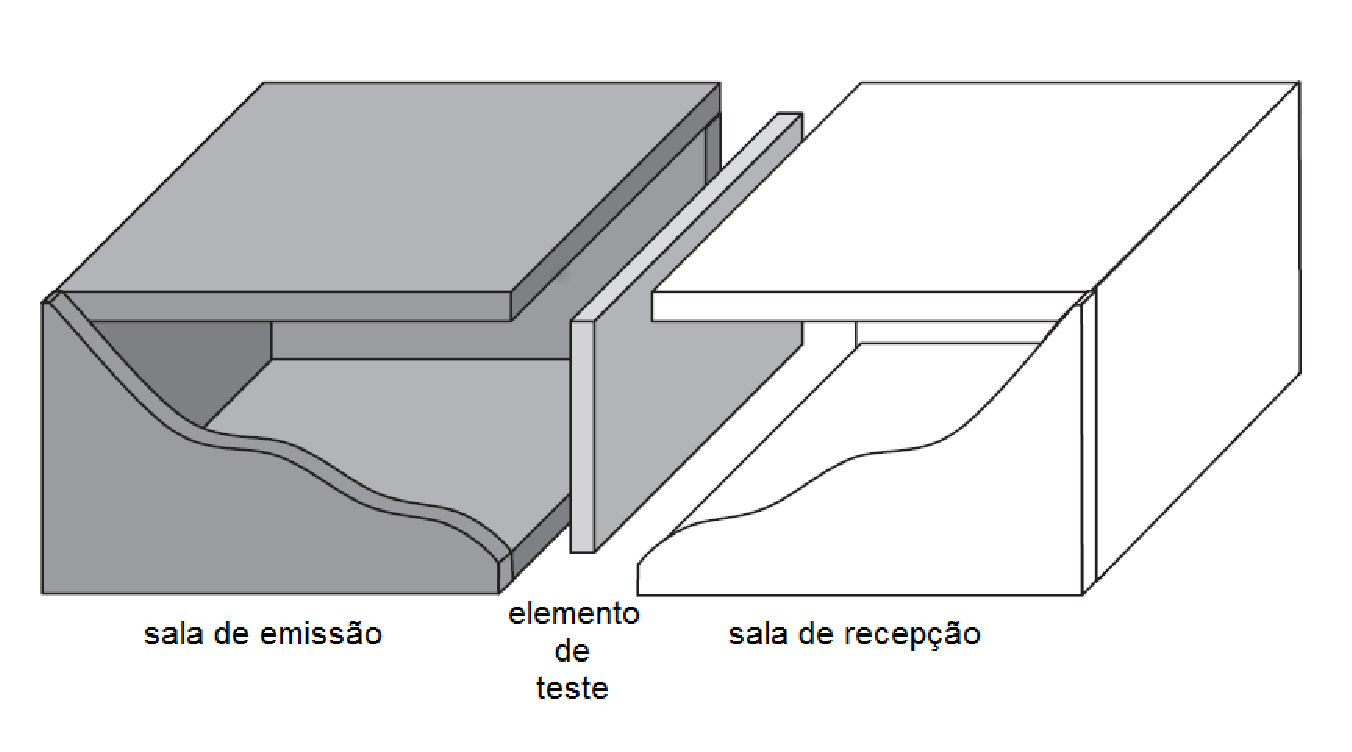
\includegraphics[scale=0.5]{teoria_1.eps}
	%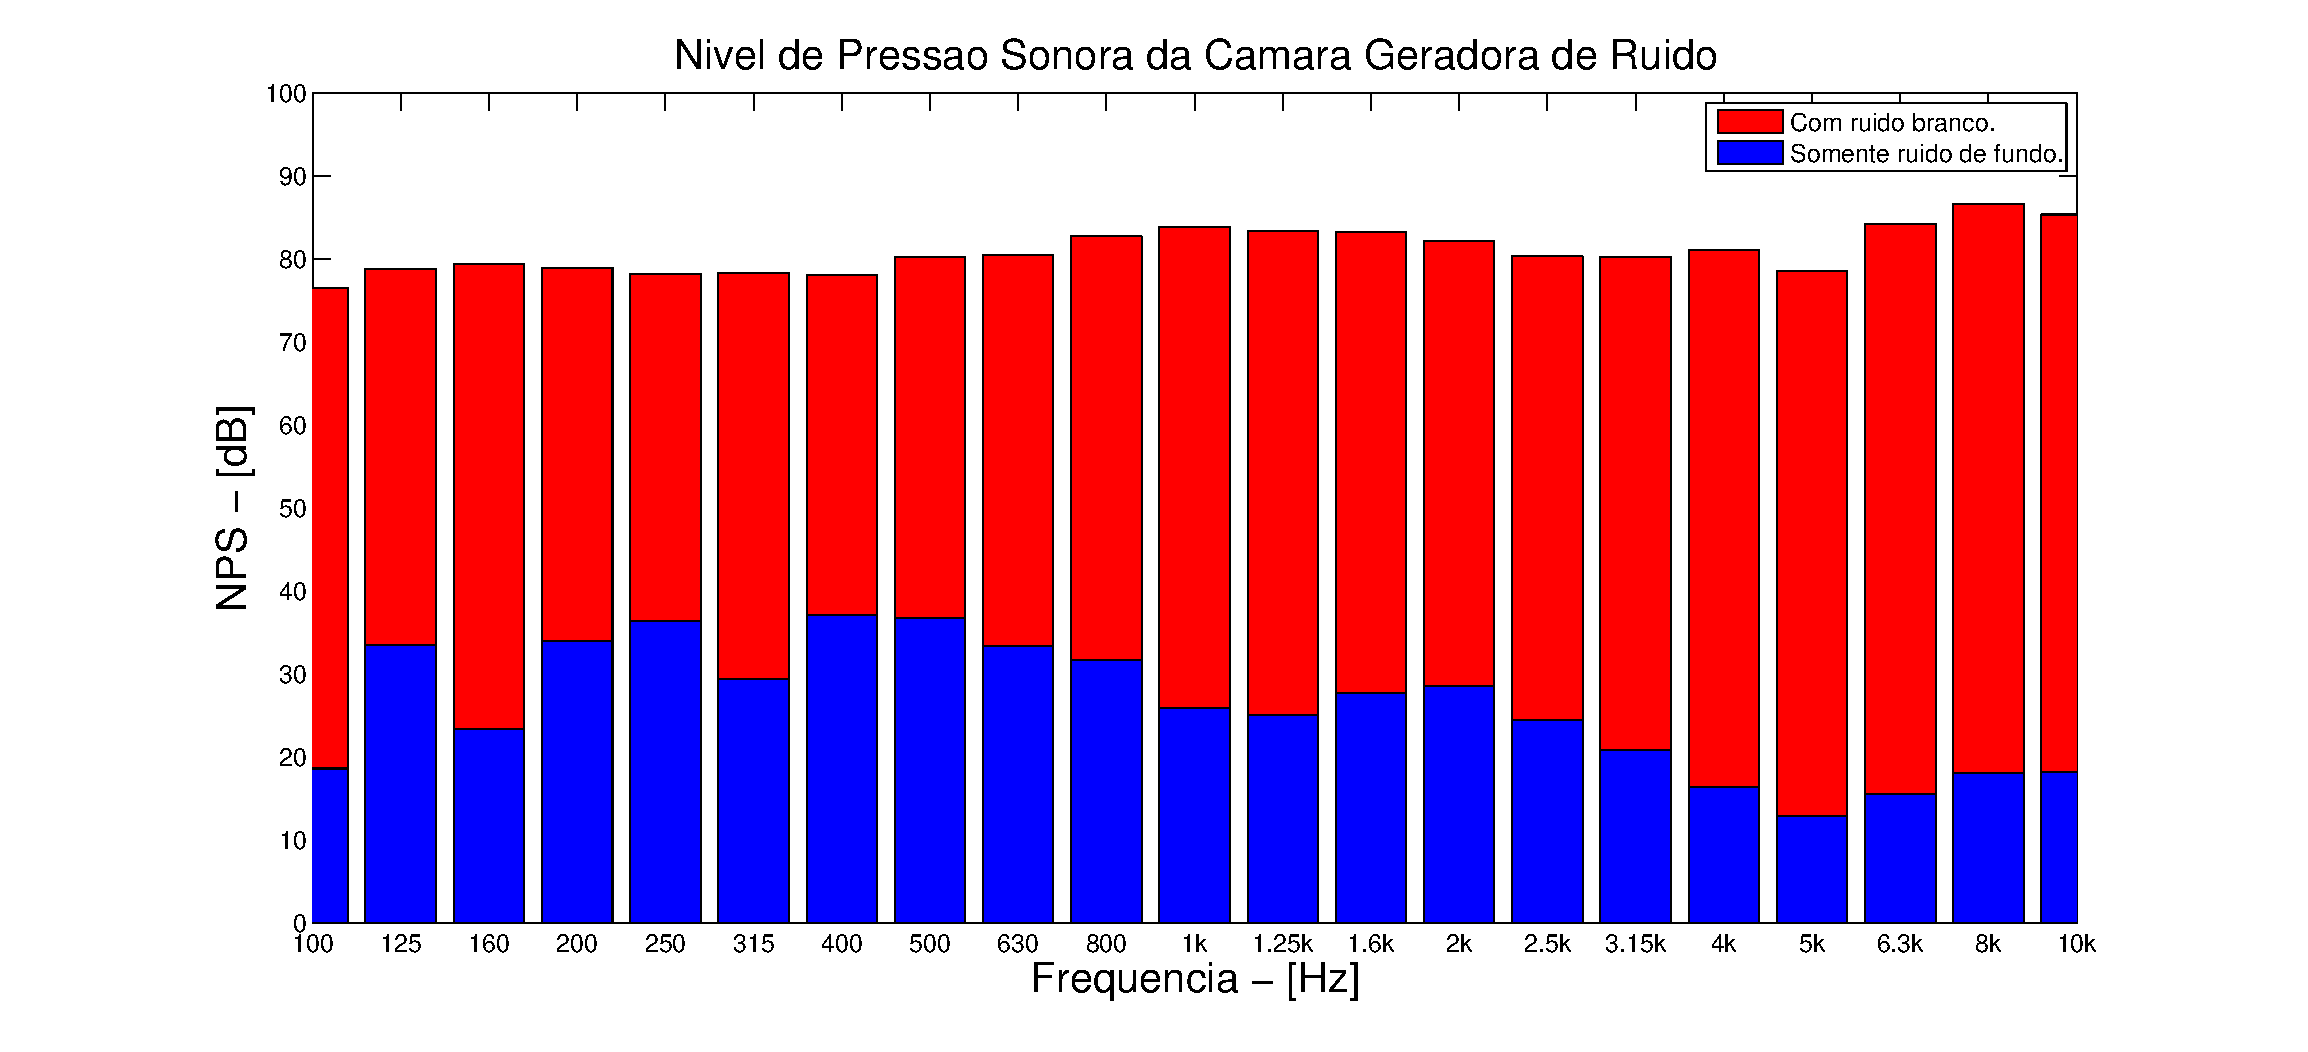
\includegraphics[width=40cm,height=40cm,keepaspectratio]{codigo/pressao_sonora_geradora.eps}
	\caption{Câmaras acústicas (emissão e recepção) separadas por um elemento de teste de
área $S_p$. Fonte: \cite{silva2009simulaccao}}
	\label{teoria_1}
\end{figure}

A intensidade sonora incidente na superfície de transmissão nesse ambiente é dada pela equação \ref{eq1}, quando o campo difuso na sala emissora é estabelecido através de uma pressão sonora $p_{e}$.

\begin{equation}
	I_{e}=\frac{p_{e}^{2}}{4\rho c}
	\label{eq1}
\end{equation}

Por definição o coeficiente de perda de transmissão $\tau$ é definido pela razão da intensidade sonora na câmara geradora pela câmara receptora ficando na forma da equação \ref{eq2}.

\begin{equation}
	\tau=\frac{I_{trans}}{I_{inc}}
	\label{eq2}
\end{equation}

De forma logarítmica o $\tau$ é expresso como perda de transmissão sonora aérea $PT$ tal qual é expresso na equação \ref{eq3}.

\begin{equation}
	PT = 10 log_{10}\left(\frac{1}{\tau}\right)
	\label{eq3}
\end{equation}

Como a transmissão sonora é produzida somente pela placa delimitada pela área $S_p$, a potência da energia acústica na câmara geradora é dada pela equação \ref{eq4}.

\begin{equation}
	W_{geradora} = I_{geradora}S_{p}\;,
	\label{eq4}	
\end{equation}

Ou pode ser dada pela equação \ref{eq5}.
\begin{equation}
	W_{geradora} = I_{receptora}\tau S_{p}\;,
	\label{eq5}	
\end{equation}

Sabendo que a intensidade sonora na câmara receptora é equivalente a $ I=\frac{p_{e}^{2}}{4\rho c} $, a potência acústica transmitida para sala receptora é expressa pela equação \ref{eq6}.

\begin{equation}
	W_{geradora}=\frac{p_{e}^{2}}{4\rho c}\tau S_{p}
	\label{eq6}
\end{equation}

A potência sonora radiada pela parede para a sala receptora é igual a potência sonora absorvida pela mesma sala, e se esta sala também possui um campo sonoro difuso, tem-se que a potência transmitida é equivalente a potência absorvida dada pela equação \ref{eq6}.

\begin{equation}
	W_{trans} = W_{abs}=\frac{p_{r}^{2}}{4\rho c}A\;,
	\label{eq6}
\end{equation}

\noindent{onde $ A $ é a absorção sonora equivalente da sala receptora.}
Através da equivalência entre a potência sonora transmitida e absorvida pode-se obter a perda de transmissão pela equação \ref{eq7}.
\begin{equation}
	\tau = \frac{p_{r}^{2}}{p_{e}^{2}}\frac{S_{p}}{A}
	\label{eq7}
\end{equation}

Ou pode ser dado pela equação \ref{eq8}.

\begin{equation}
	PT = NPS_{e} - NPS_{r} + 10log_{10}\left(\frac{S_{p}}{A}\right)
	\label{eq8}
\end{equation}

Segundo \cite{silva2009simulaccao} e \cite{lenzi2009modelos} o coeficiente de absorção $A$ pode ser calculado por duas formas. A primeira é usado o tempo de reverberação da sala receptora dada pela equação \ref{eq9}, tal qual $V$ é o volume da câmara e $T_{60}$ é o tempo de reverberação da câmara. A segunda, expressa pela formula \ref{eq10}, é usando a diferença da potência de referência da fonte e o nível de pressão da fonte de referência dentro câmara.

\begin{equation}
	A = \frac{0,161V}{T_{60}}
	\label{eq9}
\end{equation}

\begin{equation}
	log_{10}A = 6,2 + NWS_{referencia} - NPS_{referencia}	
	\label{eq10}
\end{equation}

\chapter{Experimento e Equipamentos}\label{descricao}

Para realizar as medições utilizou-se os seguintes instrumentos:

\begin{itemize}
	\item dois microfones;
	\item um calibrador de microfone;
	\item dois rotating boom;
	\item um computador
	\item um analisador de sinais modelo SCADAS da LMS;
	\item uma placa de teste (1800 mm x 1130 mm x 2 mm);
	\item uma fonte sonora;
	\item um amplificador de potência;
	\item uma fonte Sonora de referência.
\end{itemize}

E o esquemático das câmaras I e II, geradora e receptora respectivamente, foi constituída de acorda com a figura \ref{experimento_1}.

\begin{figure}[h]
	\centering
	%\hspace{-4.5cm}
	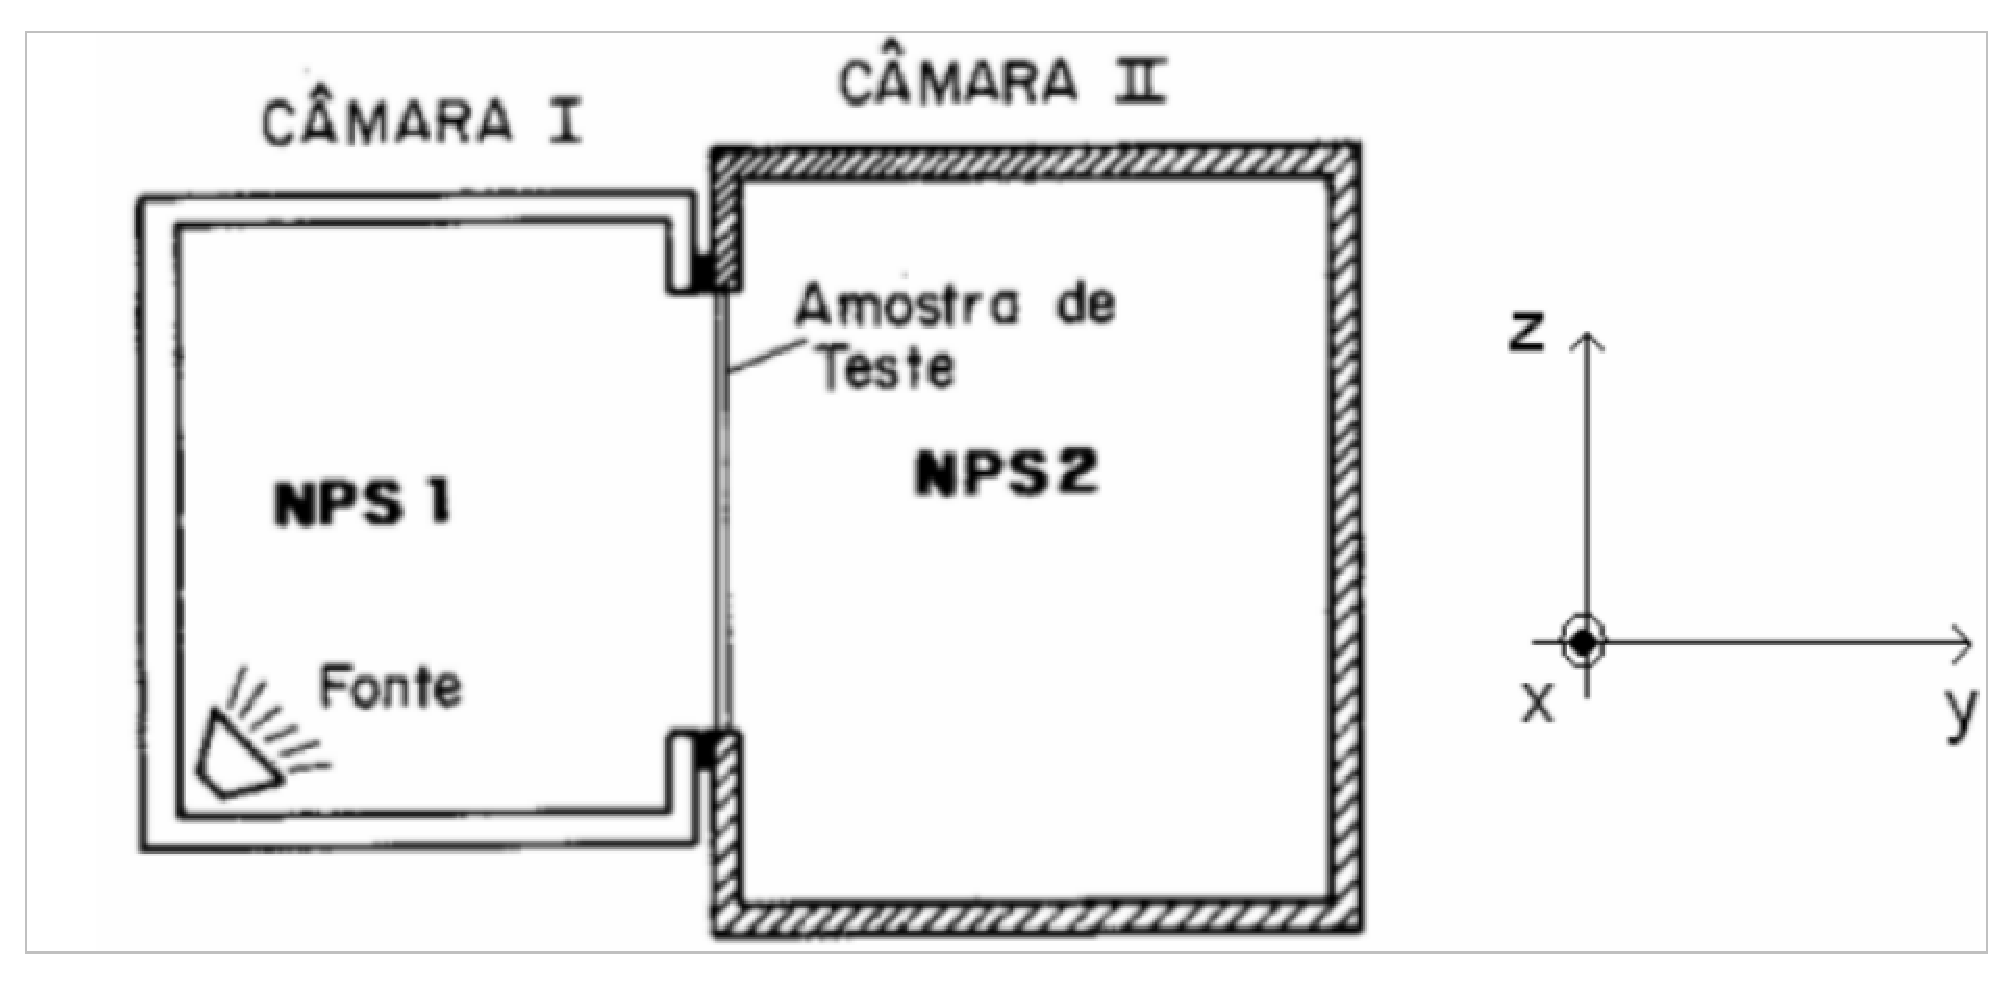
\includegraphics[scale=0.28]{imagem_3.eps}
	%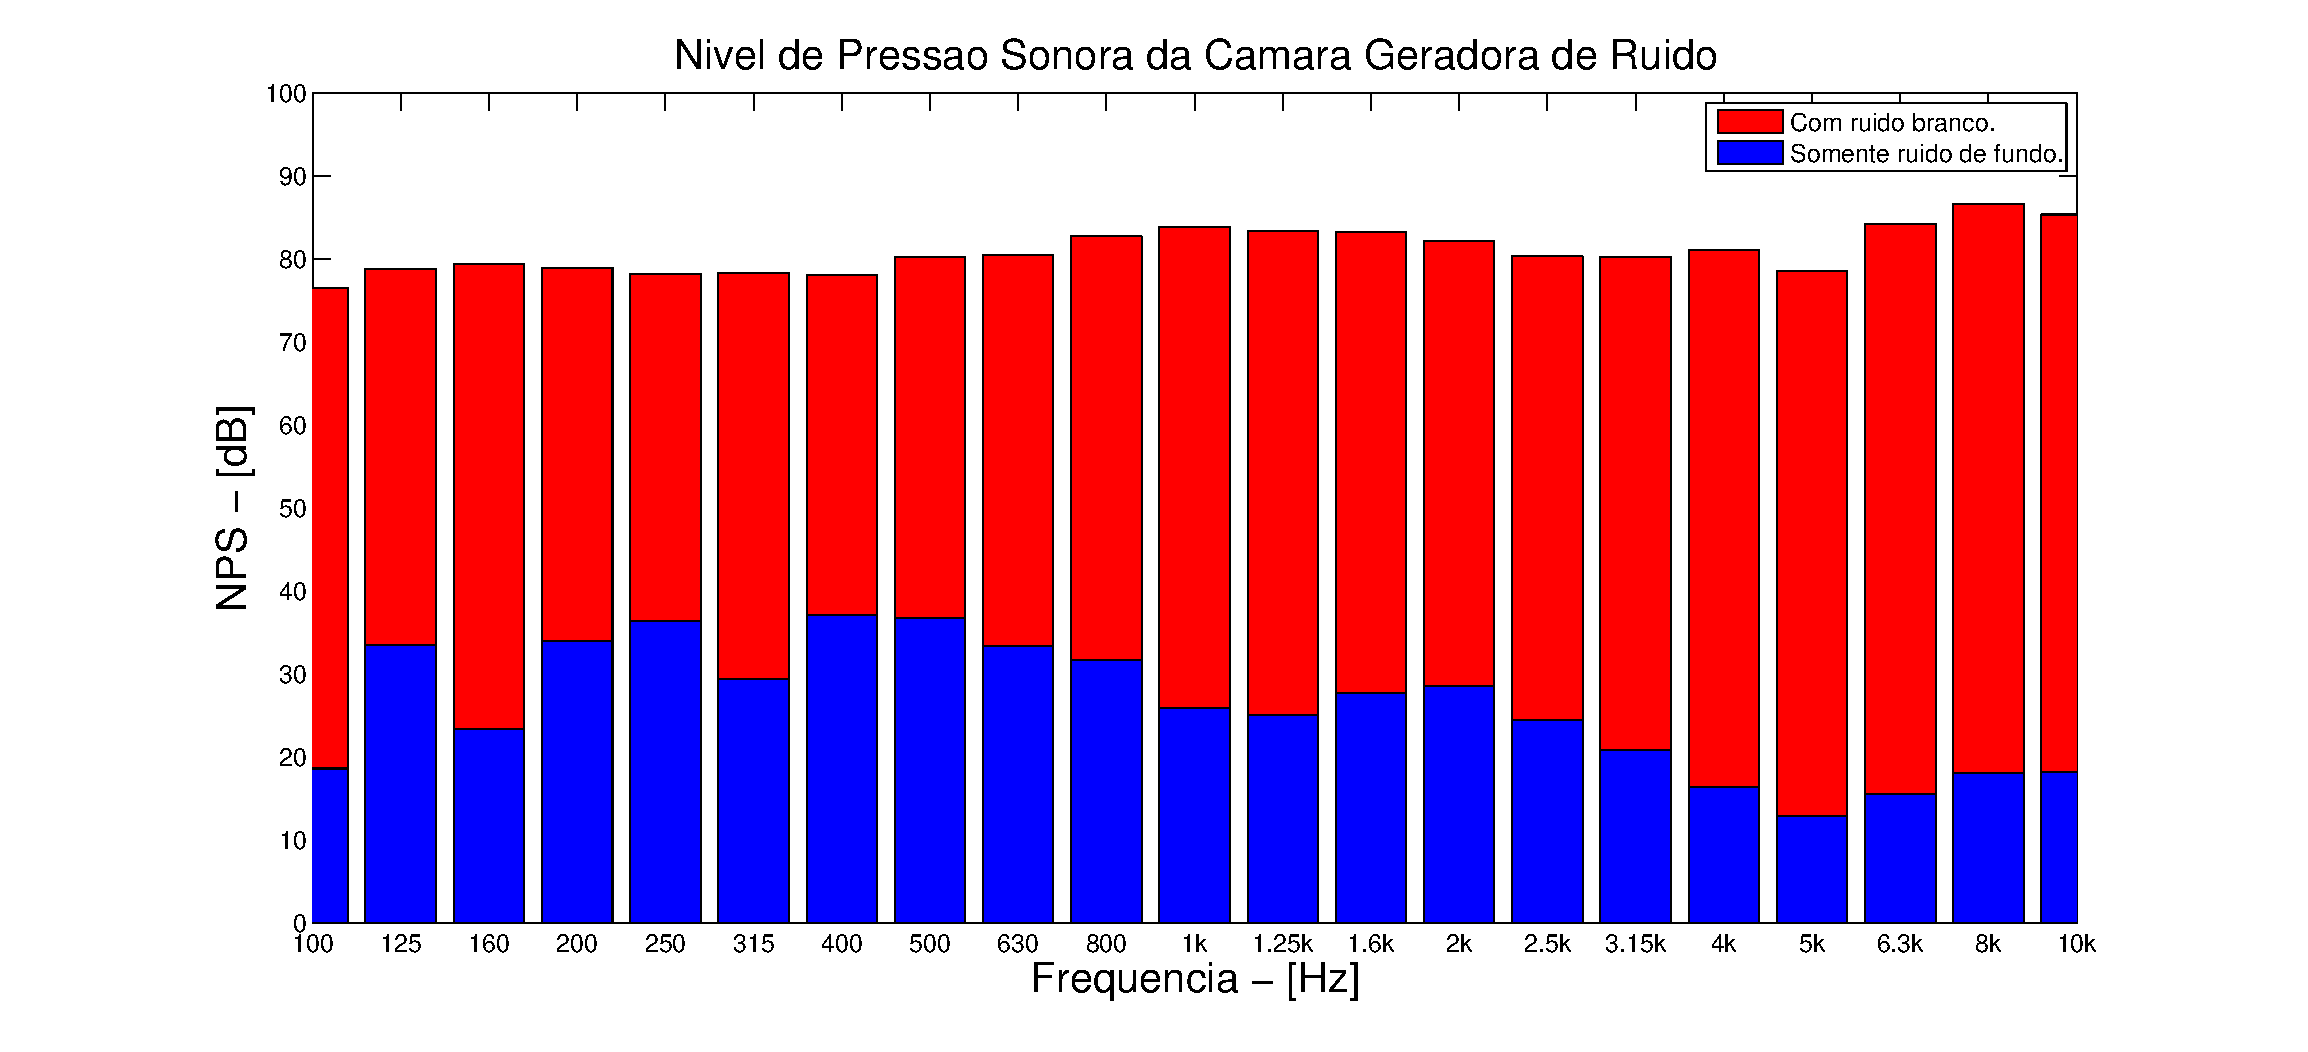
\includegraphics[width=40cm,height=40cm,keepaspectratio]{codigo/pressao_sonora_geradora.eps}
	\caption{Esquemático do acoplamento das camaras I e II. Fonte: \cite{silva2009simulaccao}}
	\label{experimento_1}
\end{figure}

\newpage
Segue as dimensões das câmaras I e II na figura \ref{experimento_2}.

\begin{figure}[h]
	\centering
	%\hspace{-4.5cm}
	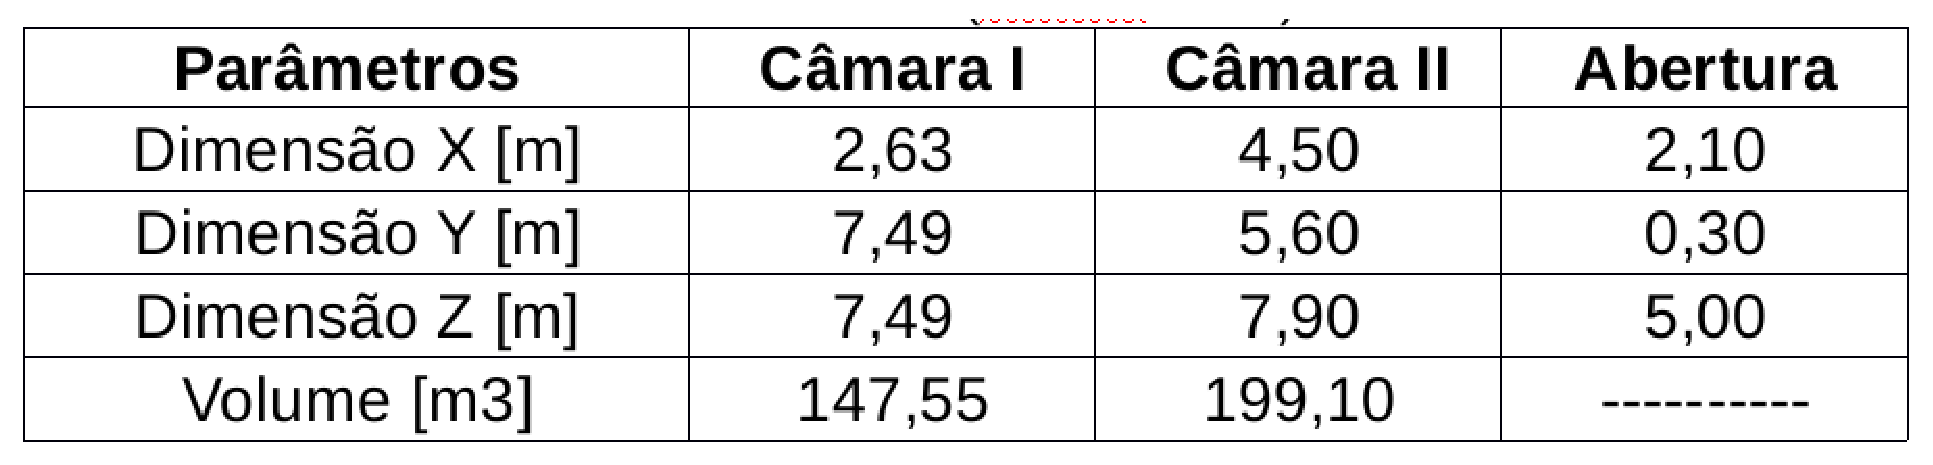
\includegraphics[scale=0.35]{imagem_4.eps}
	%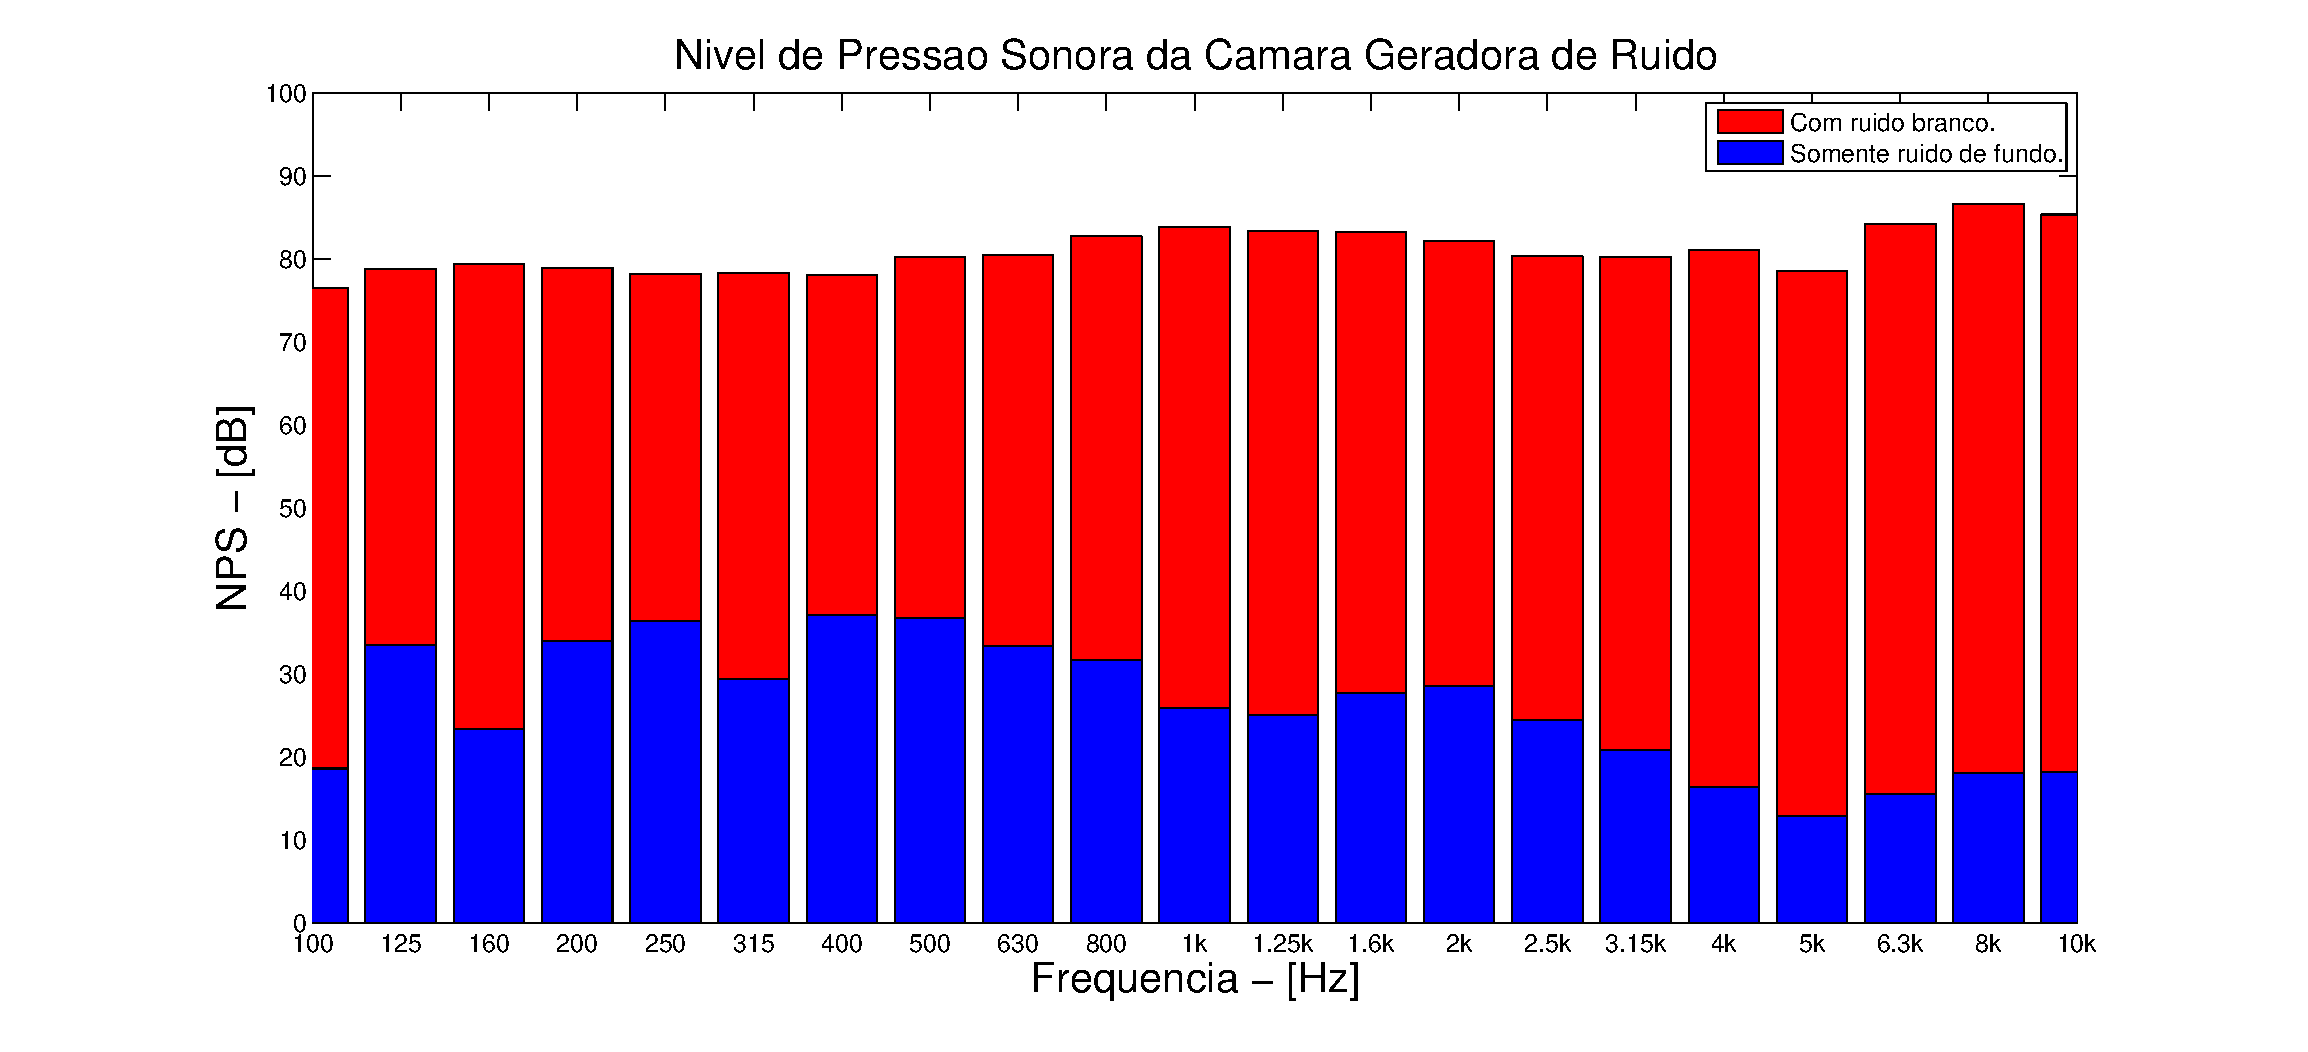
\includegraphics[width=40cm,height=40cm,keepaspectratio]{codigo/pressao_sonora_geradora.eps}
	\caption{Dimensões das câmaras I e II. Fonte: \cite{silva2009simulaccao}}
	\label{experimento_2}
\end{figure}

Segue os tempos de reverberação das câmaras I e II na figura \ref{experimento_3}.
\begin{figure}[h]
	\centering
	%\hspace{-4.5cm}
	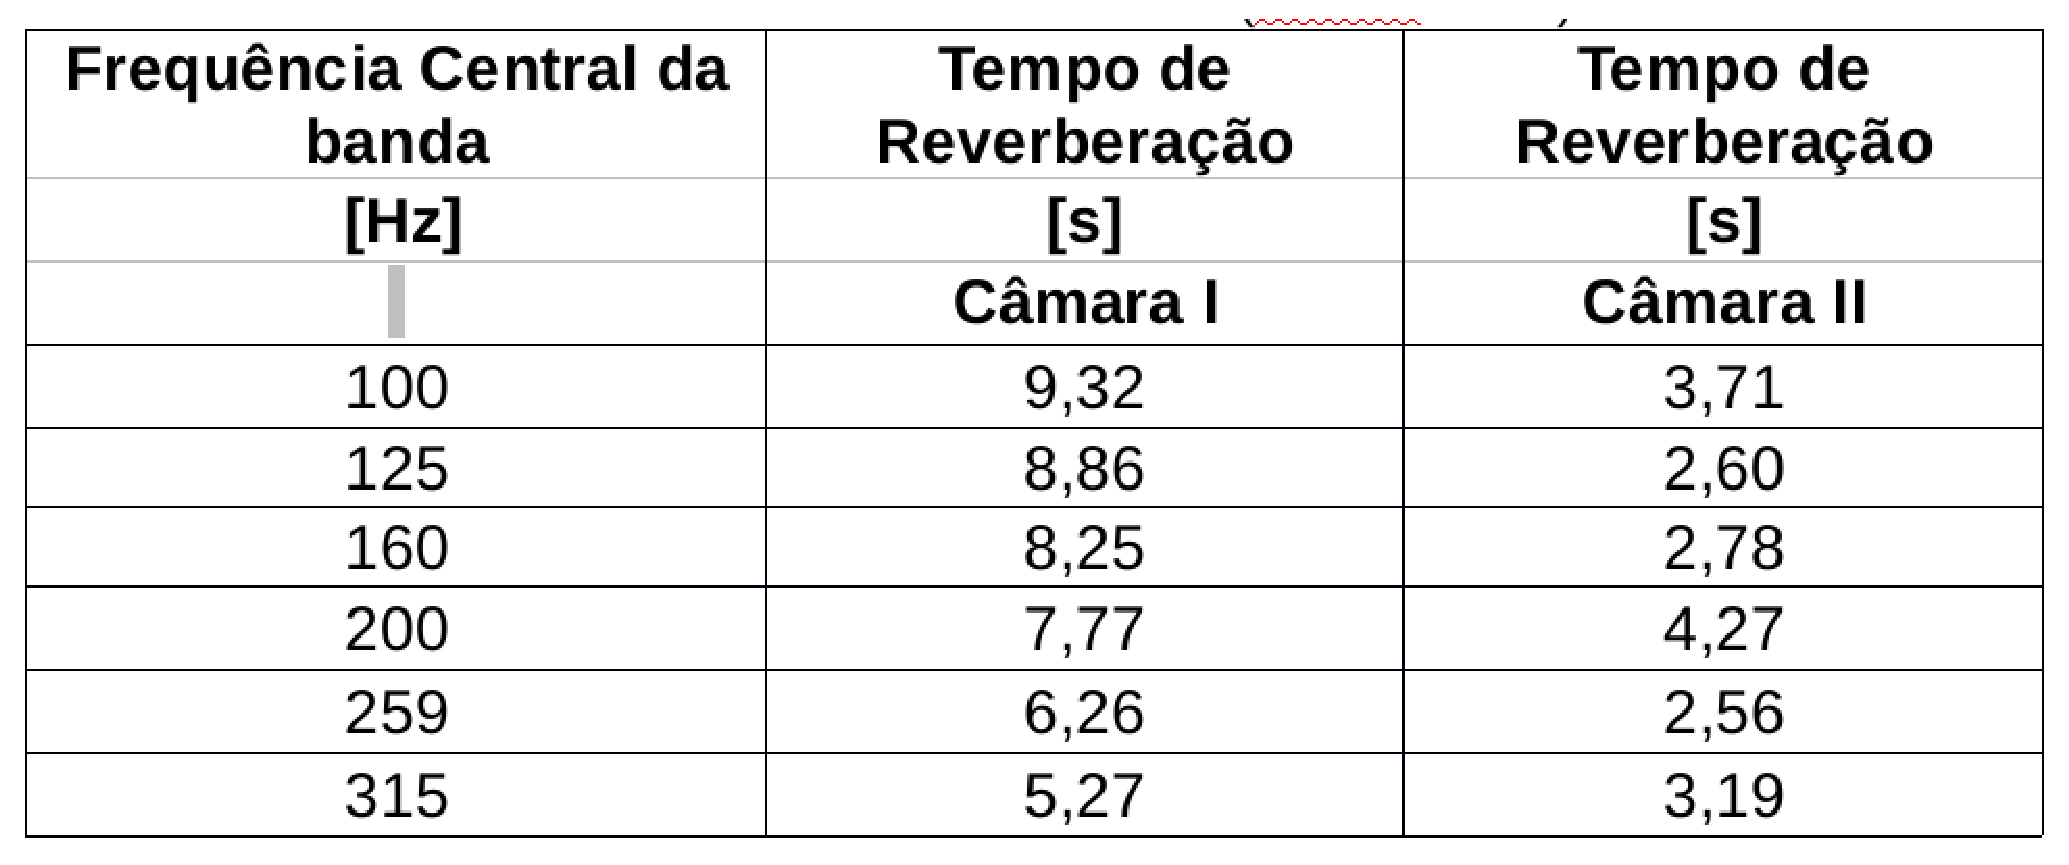
\includegraphics[scale=0.35]{imagem_5.eps}
	%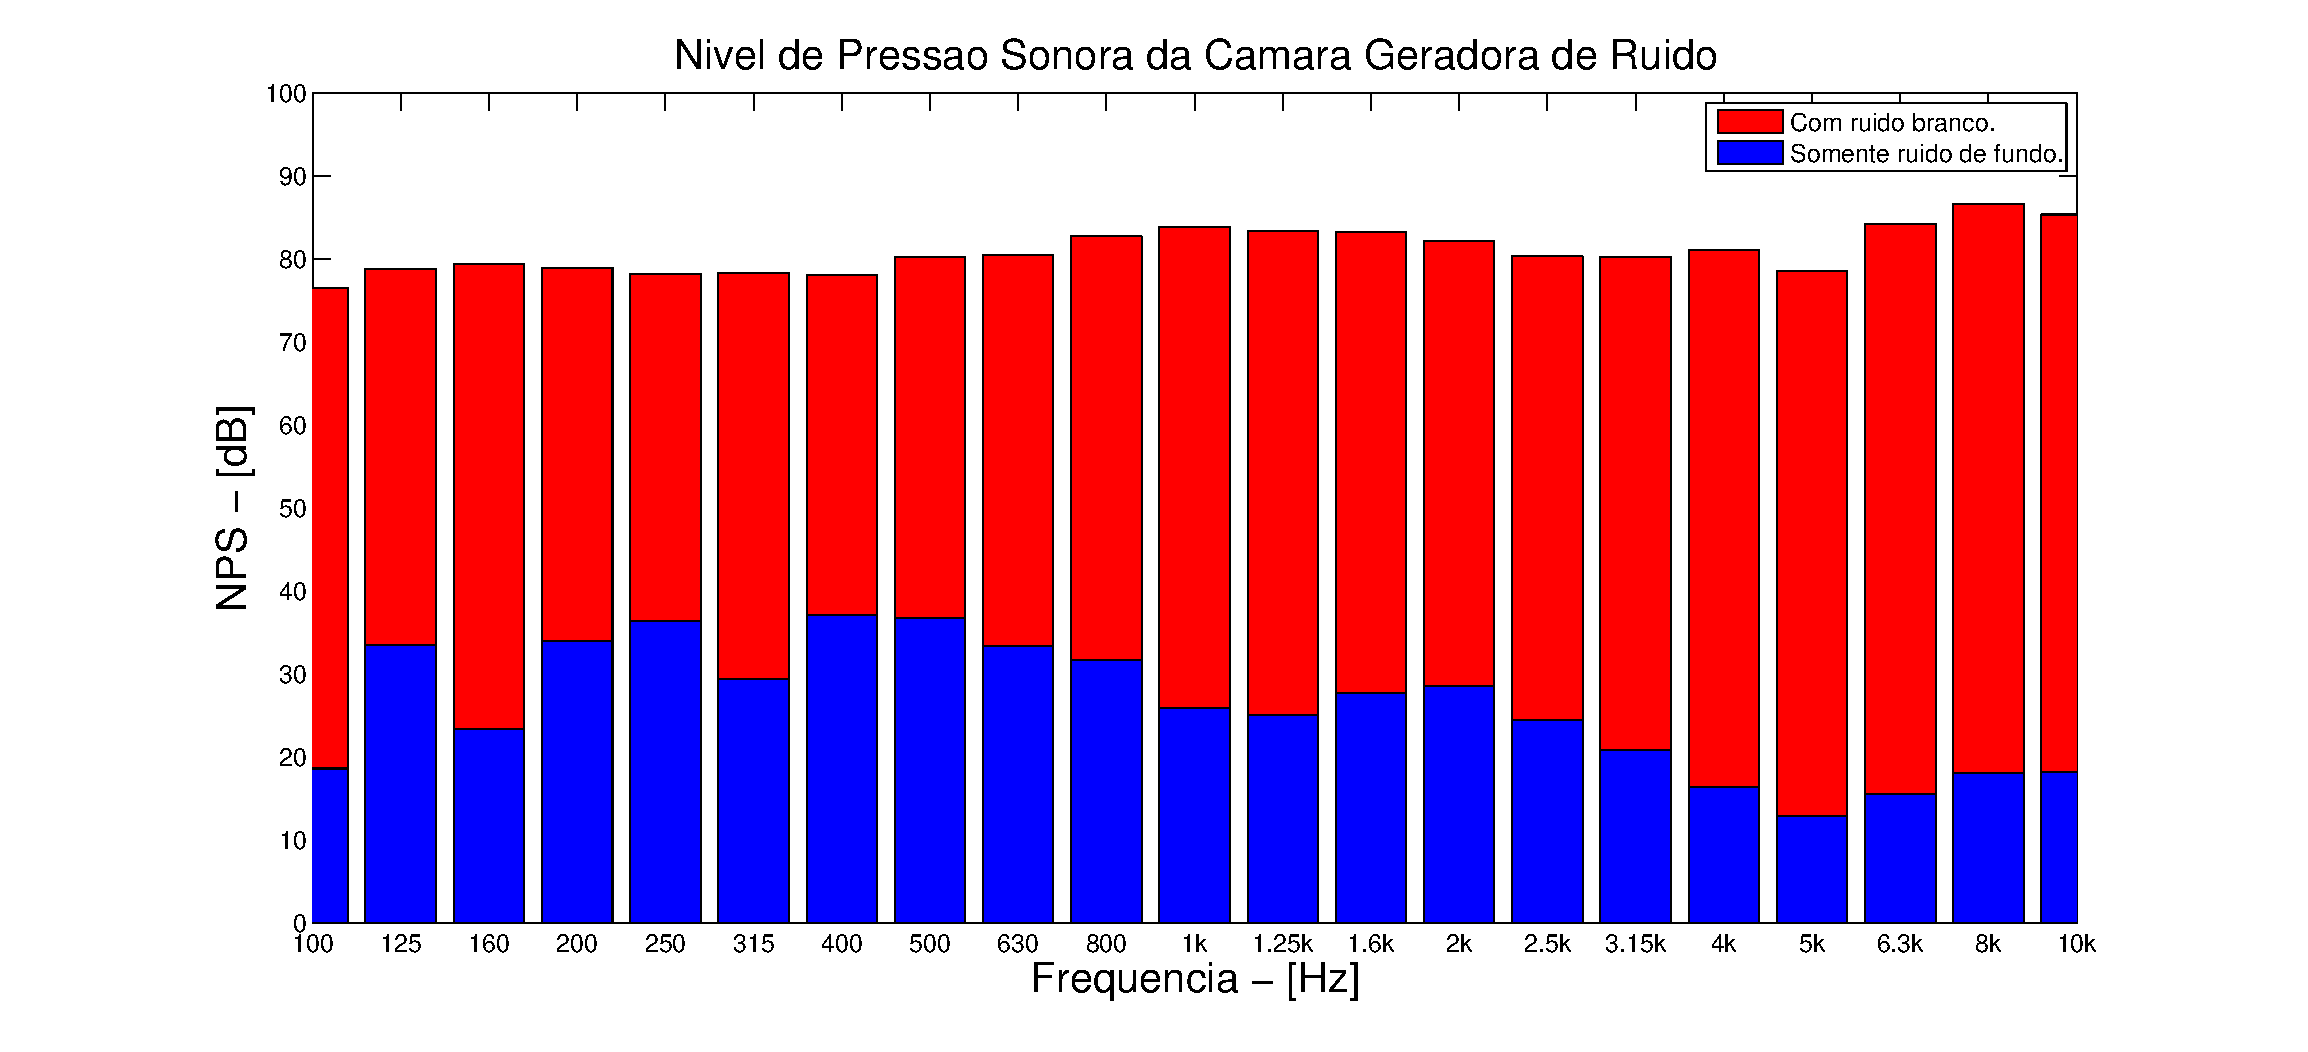
\includegraphics[width=40cm,height=40cm,keepaspectratio]{codigo/pressao_sonora_geradora.eps}
	\caption{Tempos de reverberação das câmaras I e II. Fonte: \cite{silva2009simulaccao}}
	\label{experimento_3}
\end{figure}

\newpage
Segue disposição experimental da câmara I geradora na figura \ref{experimento_4}.
\begin{figure}[h]
	\centering
	%\hspace{-4.5cm}
	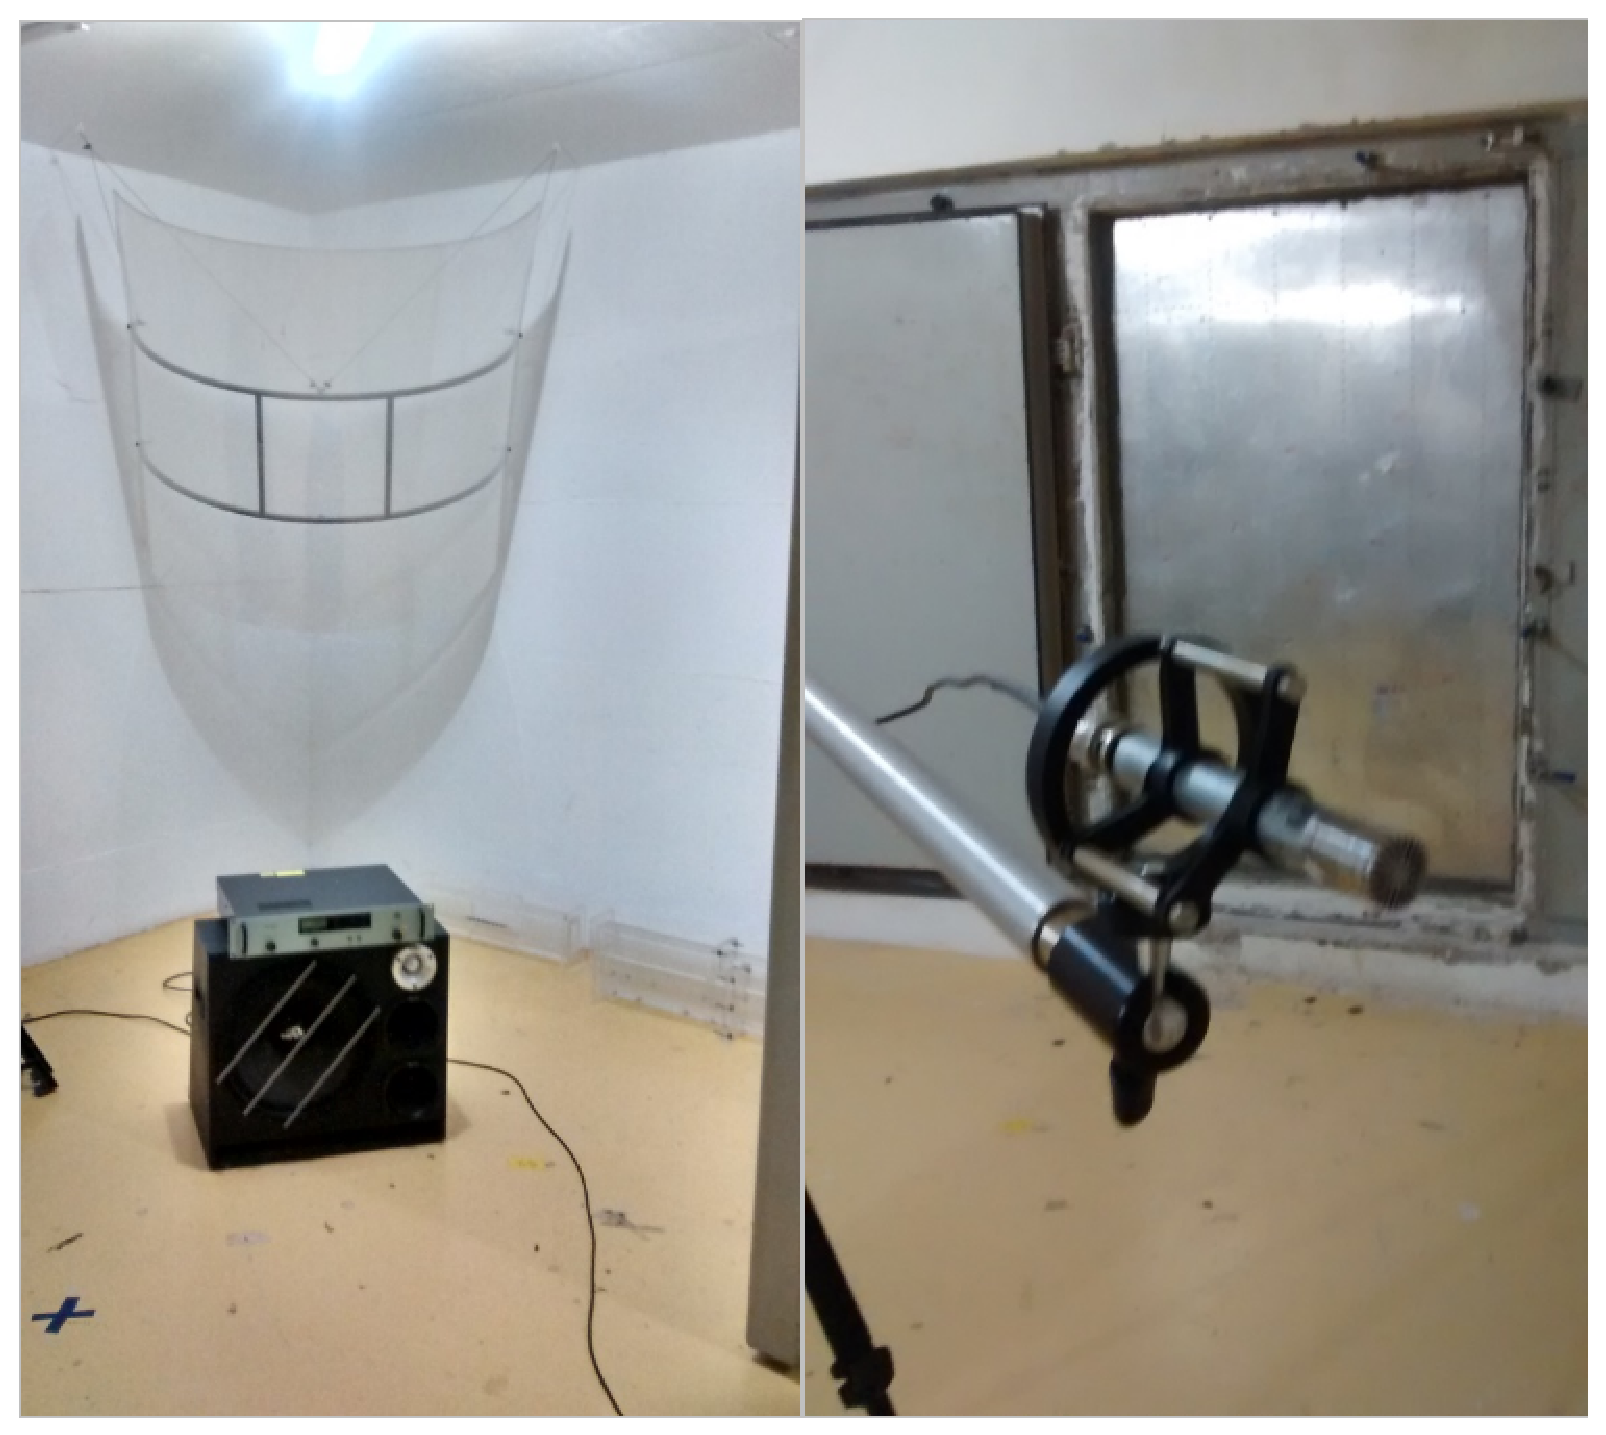
\includegraphics[scale=0.35]{imagem_2.eps}
	%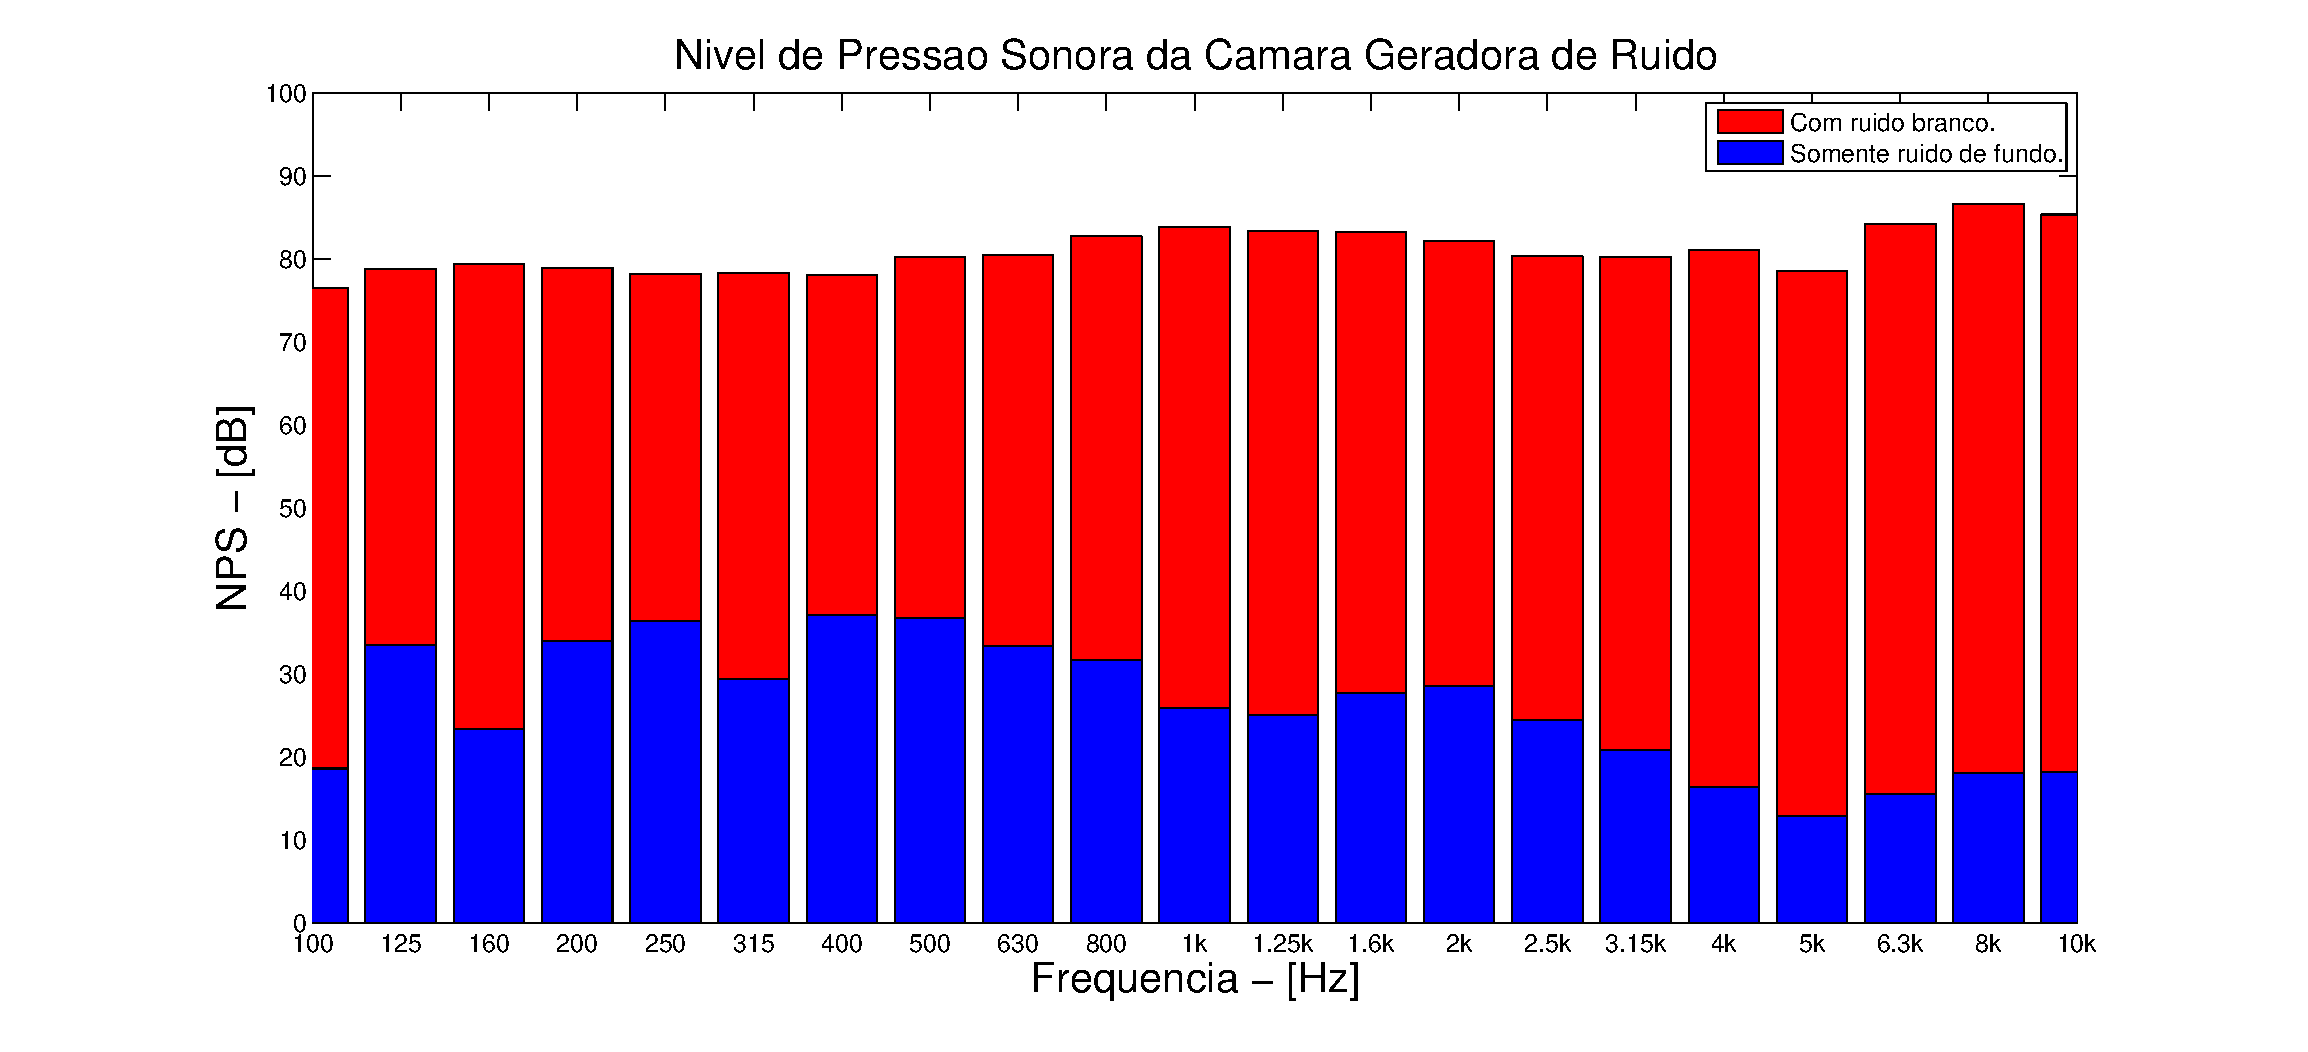
\includegraphics[width=40cm,height=40cm,keepaspectratio]{codigo/pressao_sonora_geradora.eps}
	\caption{Câmara I. Fonte: \cite{silva2009simulaccao}}
	\label{experimento_4}
\end{figure}

Segue disposição experimental da câmara I geradora na figura \ref{experimento_5}.
\begin{figure}[h]
	\centering
	%\hspace{-4.5cm}
	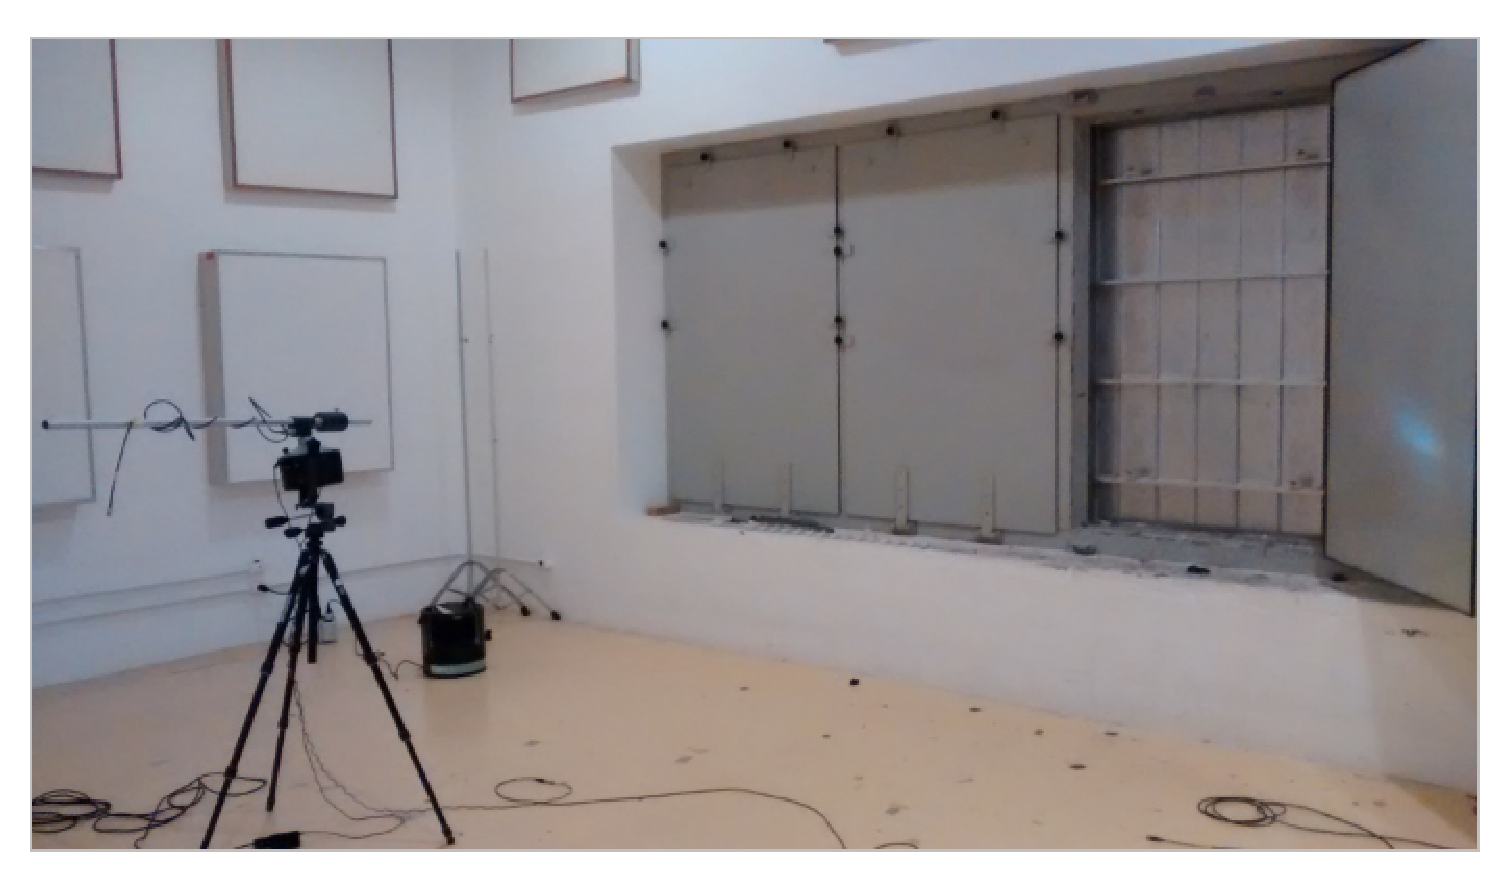
\includegraphics[scale=0.35]{imagem_1.eps}
	%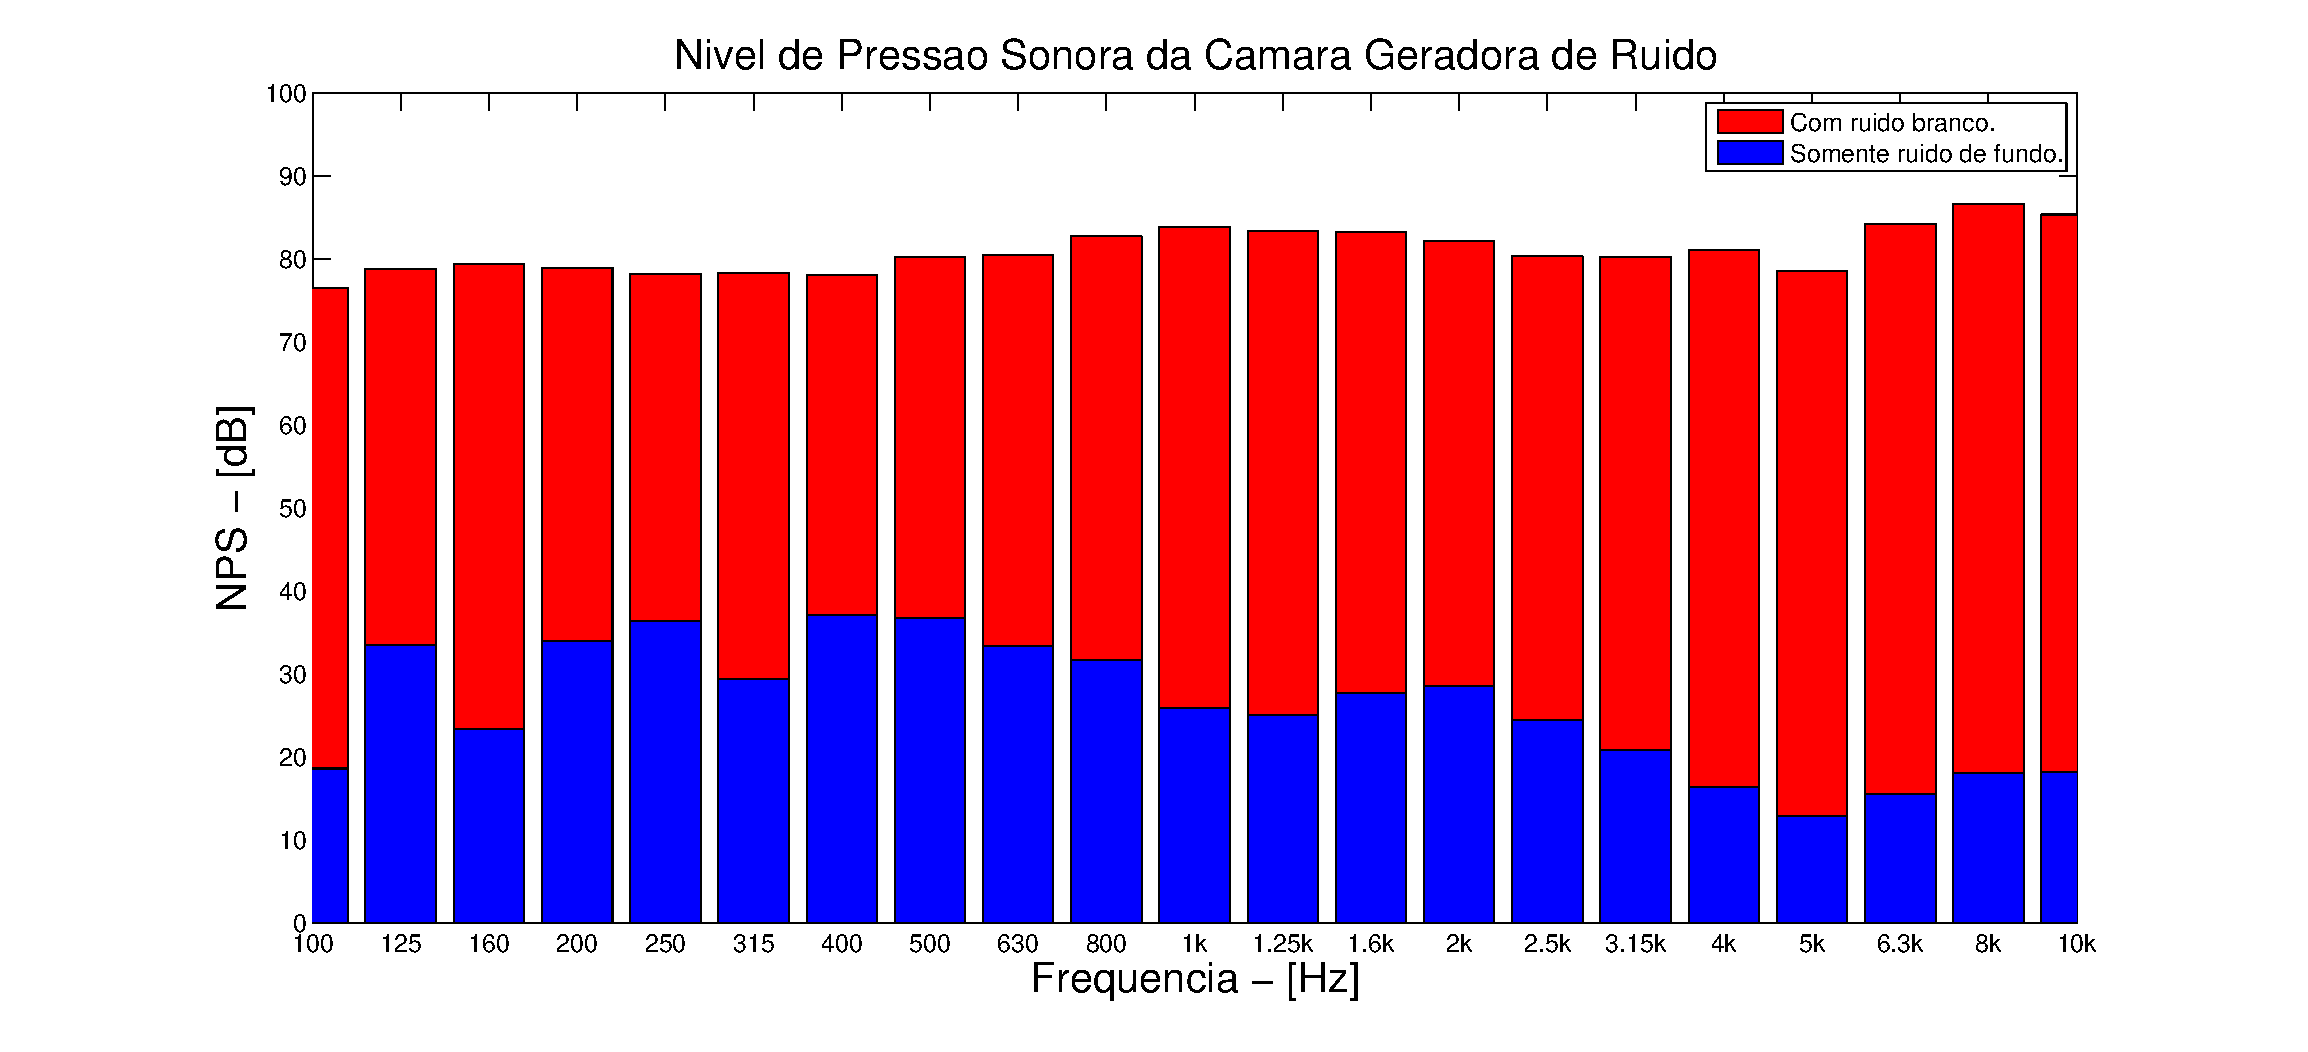
\includegraphics[width=40cm,height=40cm,keepaspectratio]{codigo/pressao_sonora_geradora.eps}
	\caption{Câmara II. Fonte: \cite{silva2009simulaccao}}
	\label{experimento_5}
\end{figure}

\chapter{Resultados}\label{resultados}

No que diz respeteito aos resultados do experimento abordado, foram consolidados o espectro de frequências do ruído branco e do ruído de fundo nas salas geradoras e receptoras respectivamente e, como resultado principal, foi extraído a perda de transmissão em relação as frequências por 2 métodos, o indireto (por comparação) e direto (por sabine, usando o tempo de reverberação da câmara).

\begin{figure}[h]
%\centering
\hspace{-4.5cm}
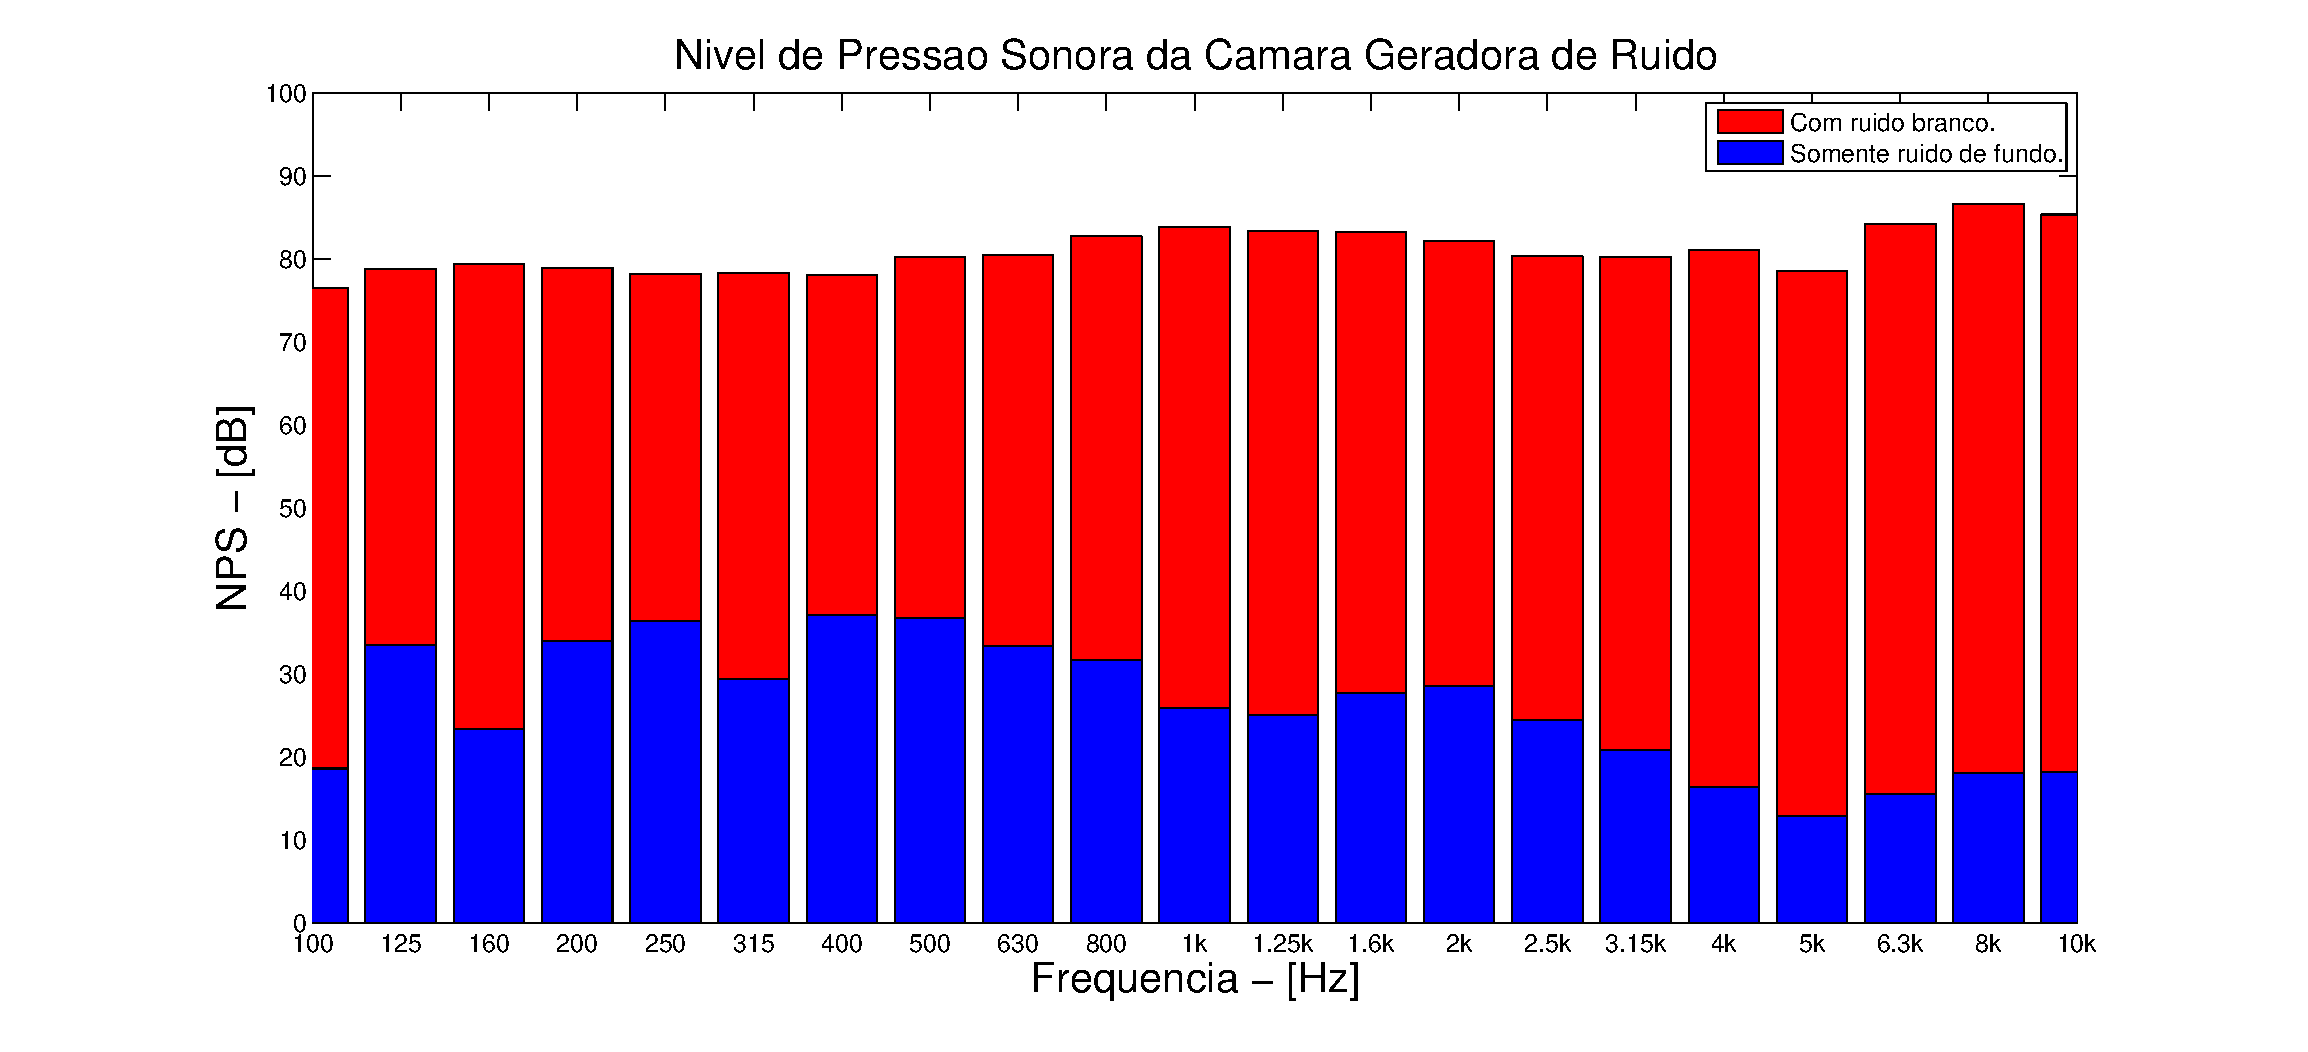
\includegraphics[scale=0.6]{codigo/pressao_sonora_geradora.eps}
%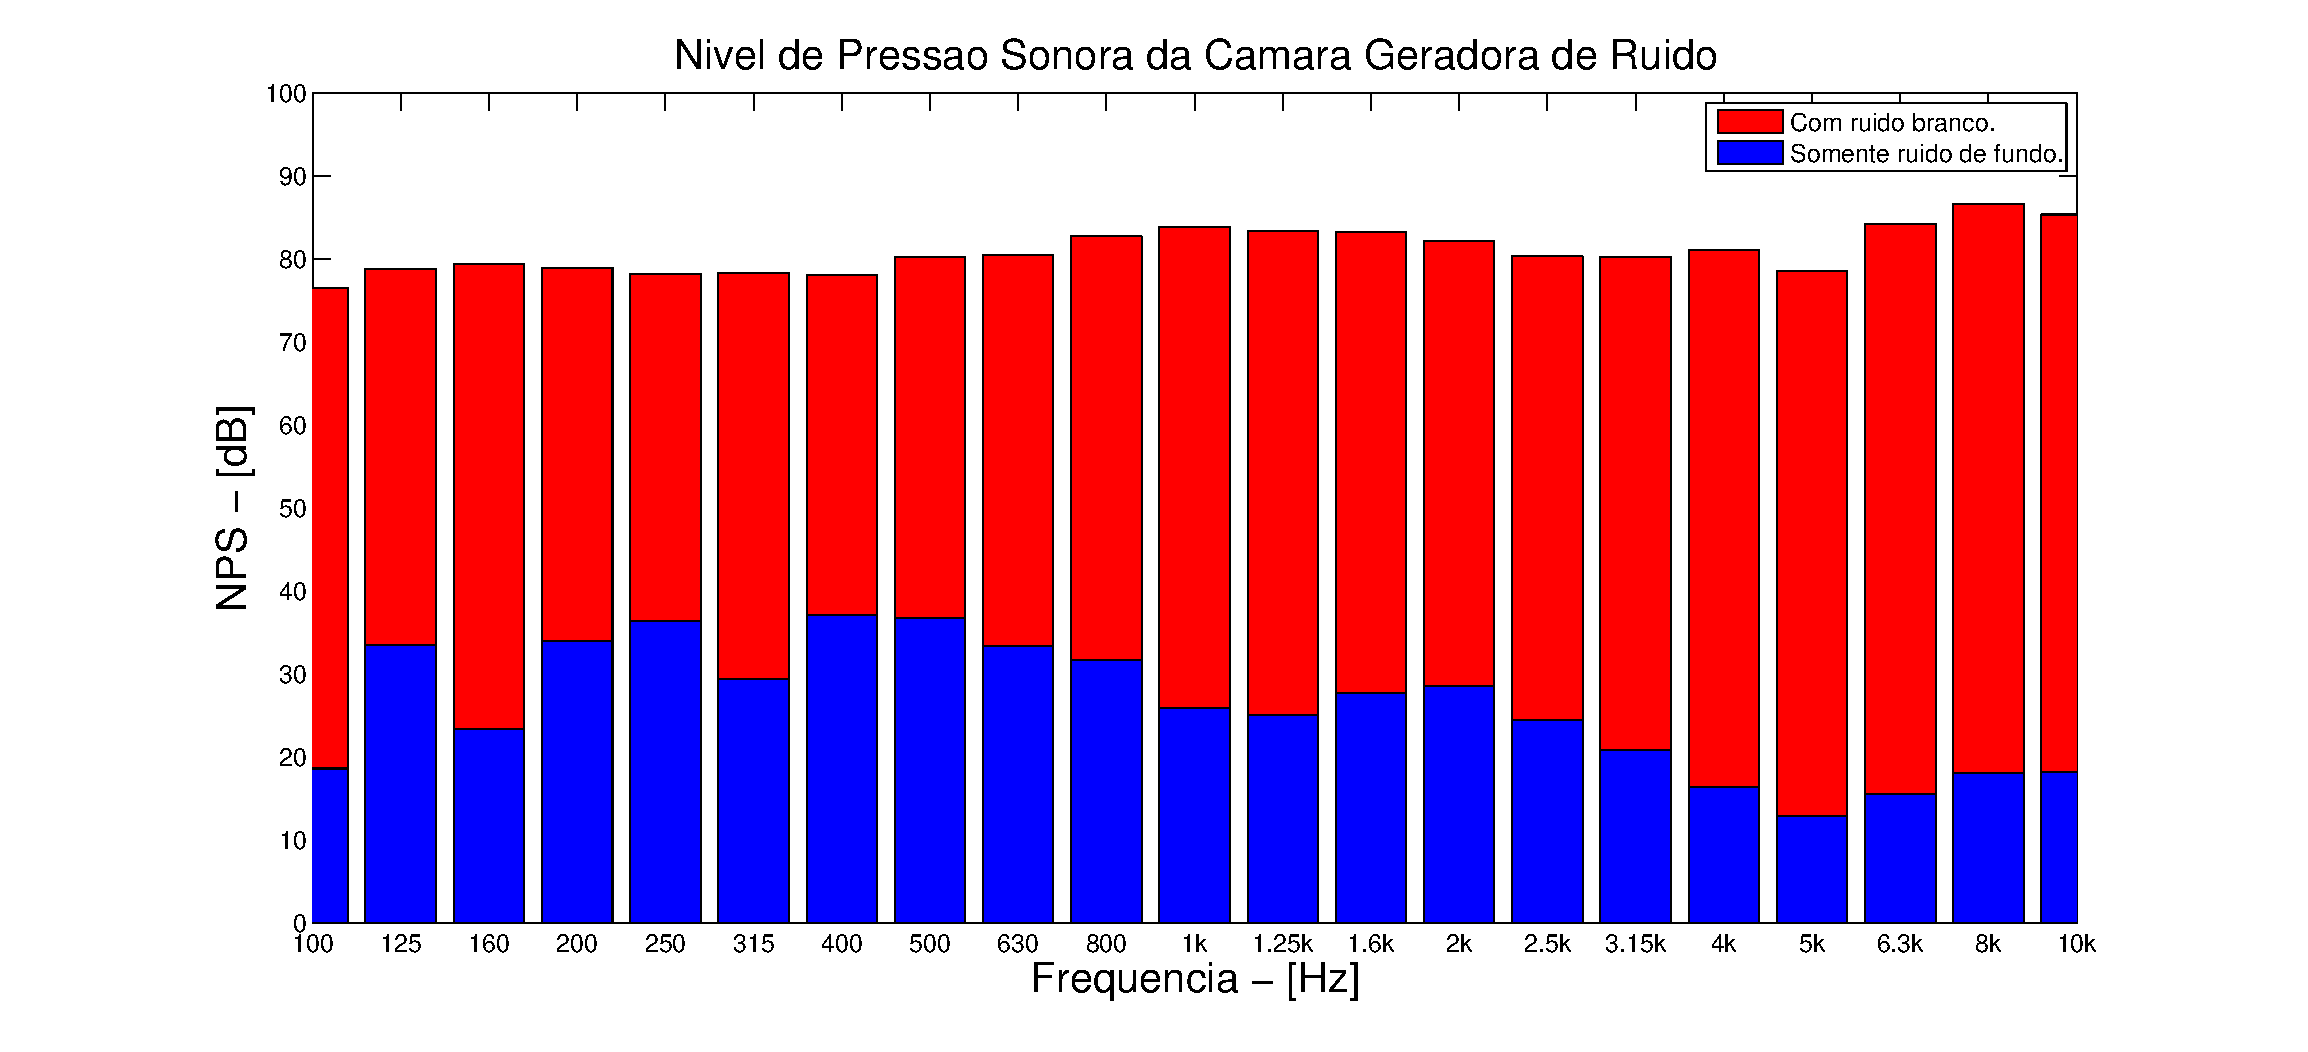
\includegraphics[width=40cm,height=40cm,keepaspectratio]{codigo/pressao_sonora_geradora.eps}
\caption{Níveis de pressão sonora na câmara geradora de ruído branco.}
\label{resultado_1}
\end{figure}

Diante do que é exposto no gráfico da figura \ref{resultado_1} é perceptível que o ruído branco se sobressaiu mais que 15 dB em relação ao ruído de fundo. Esse fato corrobora com uma medida sem necessidades de correção, pelo que é exposto em \cite{silva2009simulaccao}.

\newpage
\begin{figure}[h]
%\centering
\hspace{-4.5cm}
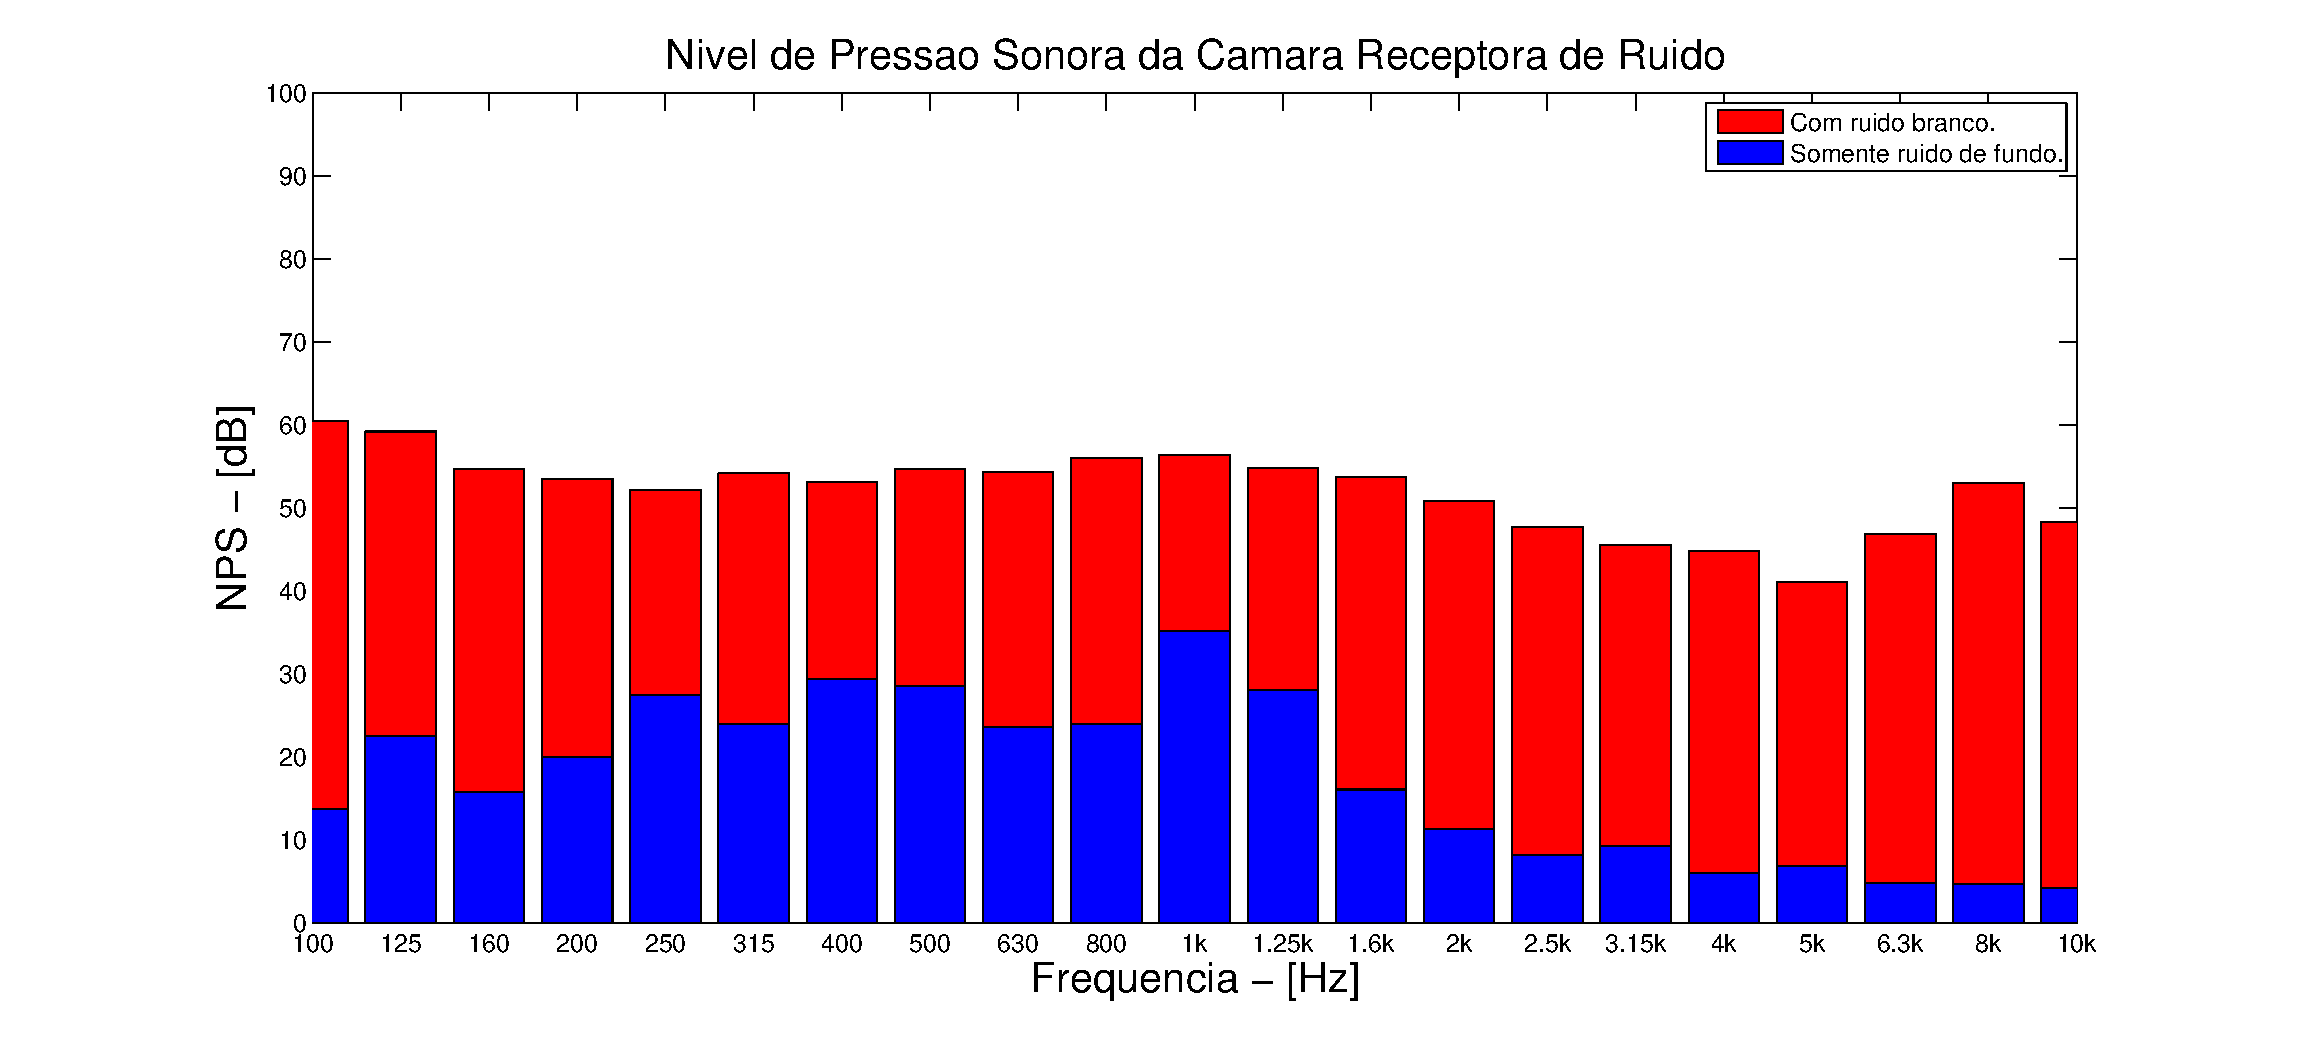
\includegraphics[scale=0.6]{codigo/pressao_sonora_receptora.eps}
\caption{Níveis de pressão sonora na câmara receptora de ruído branco.}
\label{resultado_2}
\end{figure}

Diante do que é exposto no gráfico da figura \ref{resultado_2} é perceptível que o ruído branco se sobressaiu mais que 15 dB em relação ao ruído de fundo. Esse fato corrobora com uma medida sem necessidades de correção, pelo que é exposto em \cite{silva2009simulaccao}.

\newpage
\begin{figure}[h]
%\centering
\hspace{-4.5cm}
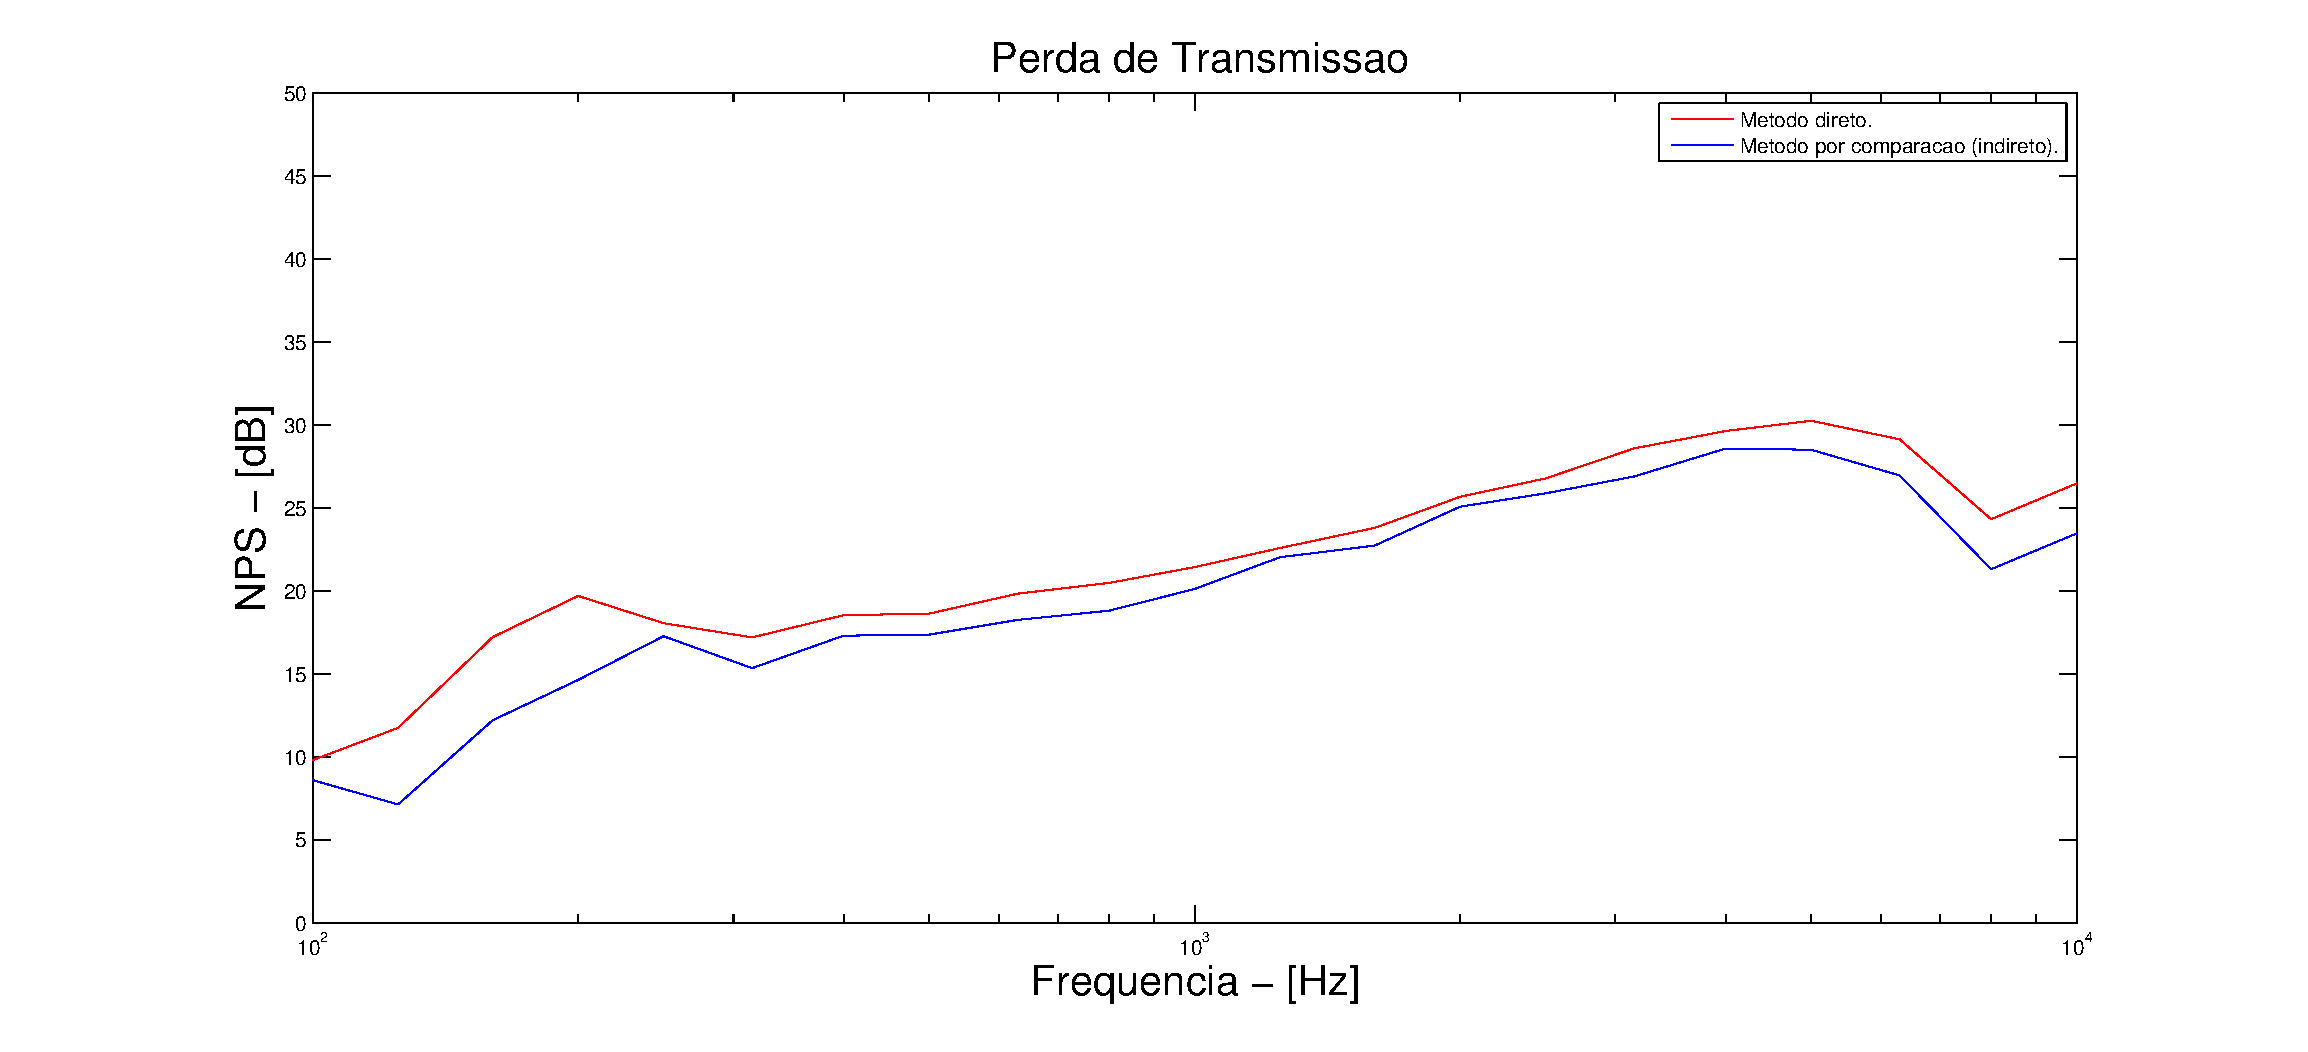
\includegraphics[scale=0.6]{codigo/perda_transmissao.eps}
\caption{Gráfico de perda de transmissão da placa de alumínio.}
\label{resultado_3}
\end{figure}

A figura \ref{resultado_3} mostra o resultado principal do experimento: a perda de transmissão em relação a frequência. É perceptível que, a medida que a placa é exposta para altas frequências, há uma perda maior. E esse fato corrobora com o que é medido pelo método indireto (feito por tempo de reverberação). As extremidades do gráfico, onde aparecem as curvas, dizem respeito ao regime elástico de comportamento, a parte linear diz respeito ao regime rígido da placa.


\chapter{Conclusões}\label{conclusoes}

O experimento descrito anteriormente reforçou as particularidades do uso de uma placa de alumínio naval para perda de transmissão. Observa-se que a medida que a frequência aumenta, maior é a perda de transmissão para ambos os métodos de cálculo de área de absorção: direto e indireto. Os resultados poderiam ser mais acurados com uma placa totalmente lisa.